\documentclass[12pt,thmsa]{article}

\newcommand{\proposition}[2]{{\bf Proposition #1.} {\em #2}}
\usepackage{natbib}
\usepackage[pdftex]{graphicx}
\usepackage{amssymb}
\def\qed{\hfill \quad \vrule height4.17pt width4.17pt depth0pt} 
\newenvironment{proof}[1][Proof]{\noindent \textbf{#1:} }{\qed}

\begin{document}

\thispagestyle{empty}

\begin{center} 
{\sc ILOG\ Technical report number 03-001}

{\sc \copyright\ ILOG\ 2003 all rights reserved}
\end{center} 

\hrulefill
\vspace{6cm}

\begin{center}
{\Large {\bf Algorithms for Propagating Resource Constraints in A.I. Planning and Scheduling: Existing Approaches and New Results}} \\
\vspace{1.5cm}
{\large Philippe Laborie} \\
\vspace{0.7cm}

ILOG\ Gentilly \\
9, rue de Verdun \\
94253 Gentilly

\end{center}
\newpage


\begin{abstract} 
This technical report summarizes   the main   existing approaches  to   propagate
resource constraints  in  Constraint-Based  scheduling and  identifies
some of their limitations for using them in an integrated planning and
scheduling framework. We then describe two new algorithms to propagate
resource constraints on discrete resources and reservoirs. Unlike most
of the   classical work in scheduling,  our  algorithms focus   on the
precedence relations between activities  rather than on their absolute
position in time. They are  efficient even when  the set of activities
is not completely  defined and when the time  window of activities  is
large.  These  features explain why   our  algorithms are particularly
suited  for integrated planning  and   scheduling approaches. All  our
algorithms  are   illustrated with  examples.  Encouraging preliminary
results are  reported on  pure  scheduling  problems as  well as  some
possible extensions of our framework.
\end{abstract}


\section{Introduction}

As underlined in \cite{smith00}, some tools are still missing to solve
problems that lie between pure AI  planning and pure scheduling. Until
now, the scheduling community has focused on the optimization of large
scheduling   problems involving a   well-defined set of activities. In
contrast, AI  planning research  - due to   the inherent complexity of
plan synthesis - has focused   on the selection of activities  leaving
aside the issues of optimization and the handling  of time and complex
resources.  From the  point of view of  scheduling, mixed planning and
scheduling problems have two  original characteristics. First, as  the
set of activities is not completely known beforehand,  it is better to
avoid  taking strong scheduling   commitments during the  search (e.g.
instantiating or strongly reducing   the time window of an  activity).
Secondly, most of the partial plans  handled by partial order planners
(POP) or by hierarchical  task  network planners (HTN) make  extensive
use of precedence  constraints between activities.  And  surprisingly,
until now, the conjunction of  precedence and resource constraints has
not  been deeply investigated,  even  in the scheduling field  itself.
Indeed, except for the special case of unary resources (for example in
job-shop scheduling), disjunctive  formulations of cumulative resource
constraints are  relatively  new techniques and  until now,  they were
mainly    used        for     search    control    and      heuristics
\cite{cesta2000,laborie95}. This is clearly a limitation, as POP-based
frameworks start  to   be competitive  with  recent   state-of-the-art
planning systems \cite{smith00,nguyen01} and are  recognized to be one
of the  most promising approaches  for  handling domains with activity
durations, and complex temporal and resource constraints.

This    paper  proposes some   new   algorithms  for  Constraint-Based
scheduling that  strongly exploit the relationships between precedence
and  resource  constraints and    allow  a natural  implementation  of
least-commitment planning   and   scheduling  approaches.    The first
section of  the paper describes  our scheduling model.  The second one
summarizes the state-of-the-art  scheduling propagation techniques and
explains why  most  of  them  are not satisfactory  for  dealing  with
integrated planning and scheduling. In  the next section, we  describe
the basic  structure - precedence graphs  - on which our  new proposed
algorithms   rely.    Then, we  present  two   original techniques for
propagating resource  constraints: the energy precedence algorithm and
the balance algorithm.  These algorithms have been implemented in ILOG
Scheduler, a    C++     library  for     constrained-based  scheduling
\cite{scheduler52}. The  next    two  sections  describe   how   these
propagation algorithms  can be embedded  in  a least-commitment search
procedure  and give    some  preliminary results  on  pure  scheduling
problems.  Finally, the last section  presents some extensions of  the
balance constraint: one that allows  for a stronger pruning, the other
that extends  it into a  plan generation procedure  that can be proved
sound and complete.

\section{Model and Notations}

\subsection{Activities.}  An   activity  $A$ corresponds  to  a   time
interval $[start(A), end(A))$   where $start(A)$ and  $end(A)$ are the
decision variables denoting  the start and  end time  of the activity.
We assume that time is discrete that is, the  values of $start(A)$ and
$end(A)$  are integer.   Conventionally, $start_{min}(A)$ denotes  the
current earliest start time, $start_{max}(A)$  the latest start  time,
$end_{min}(A)$  the earliest end time,   and $end_{max}(A)$ the latest
end time of activity $A$.  The duration  of activity $A$ is a variable
$dur(A)=end(A)-start(A)$. Depending on  the problem, the duration  may
be known in advance or may be a decision variable. In a mixed planning
and scheduling problem,  the  application of  a planning operator  may
result in the insertion  of an activity  or complex of activities into
the current plan.

\subsection{Temporal constraints.}  Our temporal constraint network is
represented   as a Simple   Temporal Problem \cite{dechter-all-91}.  A
temporal constraint is a constraint  of the form: $d_{min} \le t_i-t_j
\le d_{max}$ where $t_i$  and $t_j$ are   each either a constant  or a
variable representing the start   or  end time  of an  activity,   and
$d_{min}$ and $d_{max}$ are two  integer constants.  Note that  simple
precedence between activities ($d_{min}=0$, $d_{max}=+\infty$) as well
as release dates and deadlines ($t_j=0$) are special cases of temporal
constraints.

\subsection{Resources.}  The most general  class of resources we shall
consider in this paper is the reservoir resource. A reservoir resource
is a multi-capacity  resource that can  be consumed and/or produced by
the  activities.  A reservoir has an  integer maximal capacity and may
have an initial level. As an example of a  reservoir, you can think of
a fuel tank.
 
A discrete resource  is a special kind  of reservoir resource that  is
used over some  time  interval: a  certain   quantity of resource   is
consumed  at the start time of  the activity and  the same quantity is
released at its end time.   Discrete resources  are also often  called
cumulative  or sharable resources  in   the scheduling literature.   A
discrete resource has a   known  maximal capacity profile over   time.
They  allow us, for   example, to represent  a  pool of workers  whose
availability may change over time.

A unary resource is a discrete resource with unit capacity. It imposes
that all the activities requiring the same  unary resource are totally
ordered. This is typically the case of a machine that can process only
one operation at a time. Unary resources are the simplest and the most
studied resources in scheduling as well as in AI planning.

\subsection{Resource Constraints.}  A  resource constraint defines how
a given activity  $A$ will  require and affect  the  availability of a
given resource $R$.  It consists of a tuple  $<A,R,q,TE>$ where $q$ is
an  integer  decision variable  defining  the quantity of resource $R$
consumed (if $q<0$) or produced (if $q>0$) by activity $A$ and $TE$ is
a time extent that defines the time interval where the availability of
resource   $R$ is  affected  by  the execution   of activity  $A$. For
example:
\begin{itemize}
\item $<A,R_1,-1,FromStartToEnd>$ is  a  resource constraint   stating
      that  activity $A$ will   require  $1$ unit  of resource   $R_1$
      between its start time and  end time; thus, the availability  of
      $R_1$ will decrease of 1 unit at the start  time of $A$ and will
      increase of 1 unit at its end time, when $A$ releases $R_1$.
\item $<A,  R_2,  q=[2,3], AfterEnd>$  is  a resource  constraint that
      states that activity   $A$ will produce   $2$  or $3$ units   of
      reservoir (this is a decision variable  of the problem) $R_2$ at
      its end time. This will increase the availability of $R_2$ after
      the end time of $A$.
\item $<A, R_3, -4, AfterStart>$  is a resource constraint that states
      that activity  $A$ will consume $4$ units   of resource $R_3$ at
      its  start  time. This will  decrease  the availability of $R_3$
      after the start time of $A$.
\end{itemize} 

The   possible  time    extents are $FromStartToEnd$,    $AfterStart$,
$AfterEnd$,  \newline $BeforeStart$,  $BeforeEnd$,   and $Always$.  An
illustration of these  time extents is available in  the  left part of
Figure \ref{fig3}. Of course, the same activity $A$ may participate in
several resource  constraints.     On a  discrete resource,   all  the
quantities $q$ are less than  or equal to  zero. On a unary  resource,
they  all  belong to  the  set  $\{-1,0\}$.  Note that the   change of
resource availability   at the start or end   time  of an  activity is
considered to be instantaneous: continuous changes are not handled.
  
\begin{figure}
\centerline{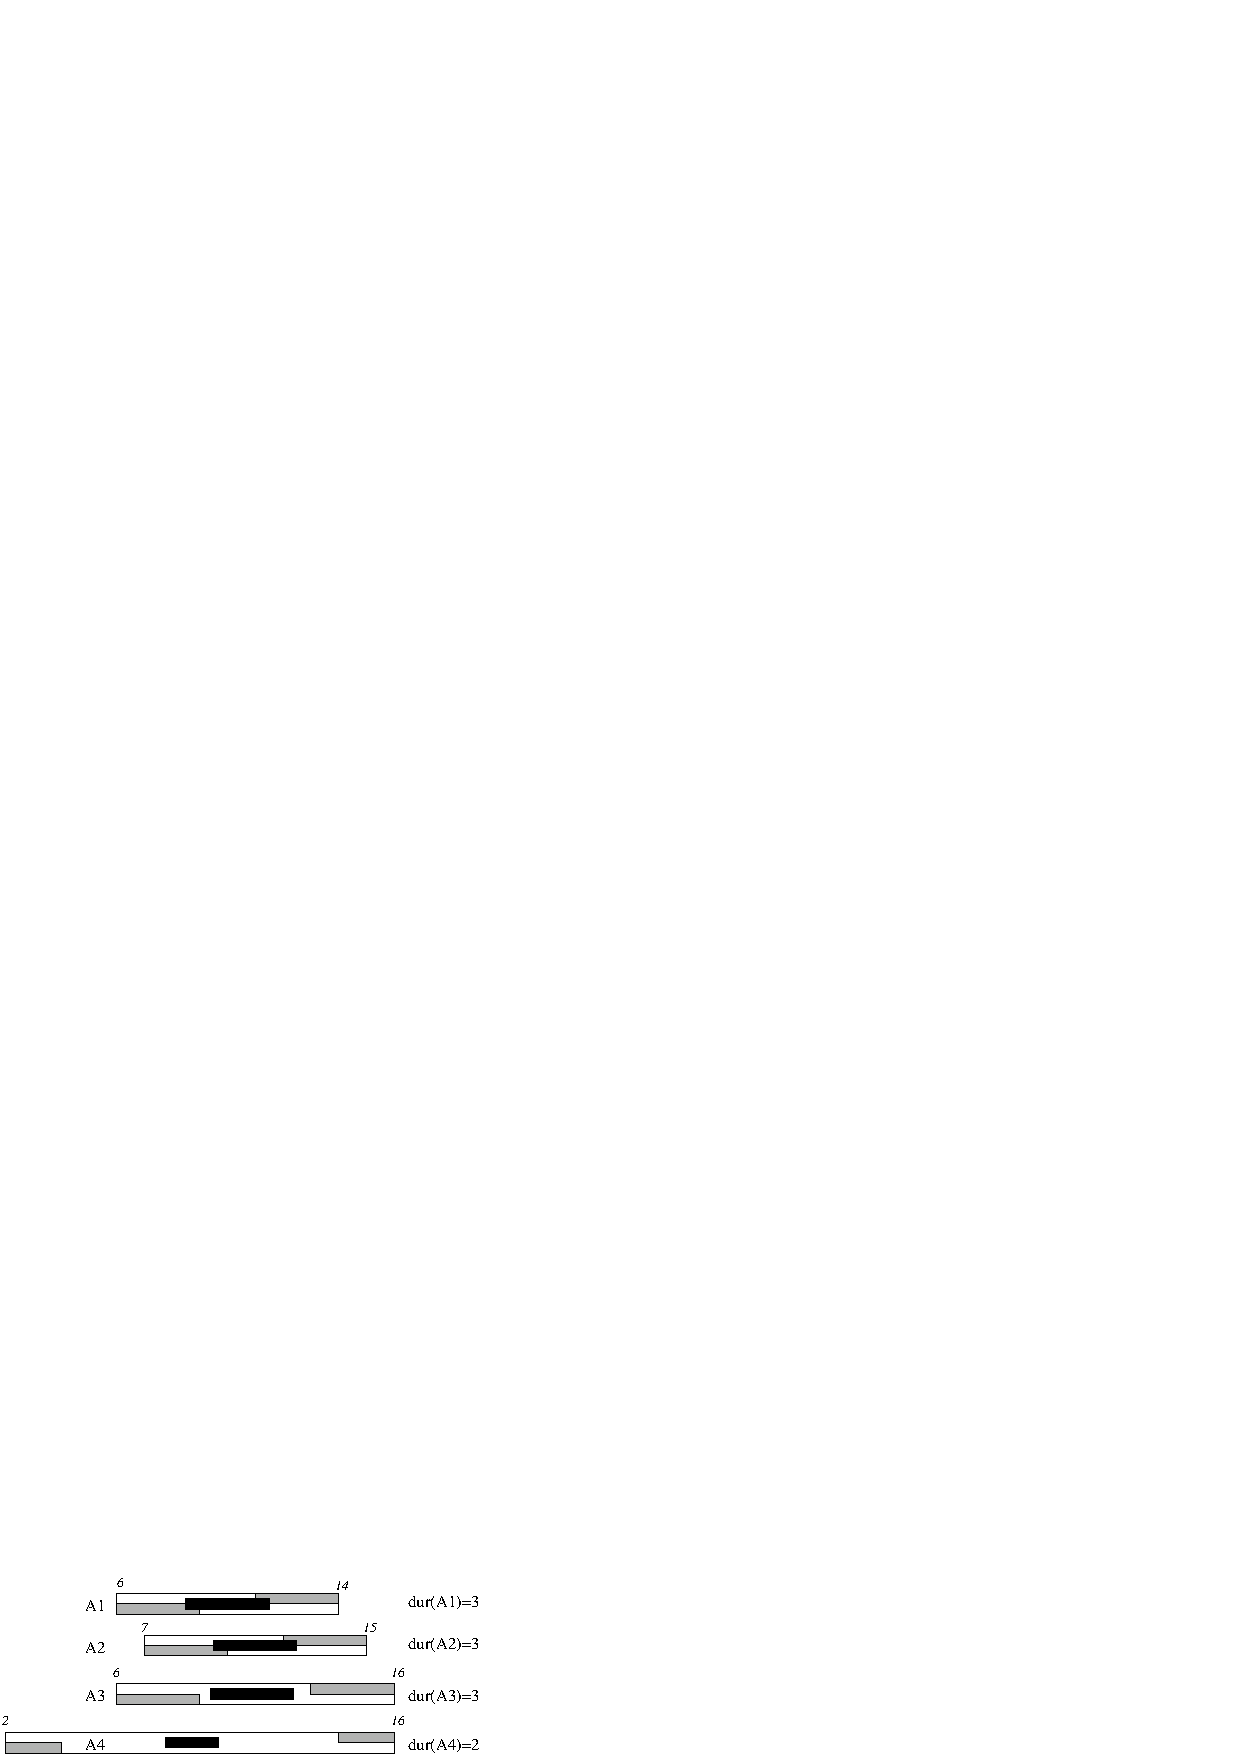
\includegraphics[width=30pc]{figures/fig3.pdf}}
\caption{Mapping between time extents and resource events}
\label{fig3}
\end{figure}

\subsection{Partial   schedule.}   We assume  in  this  paper that the
search  space consists of    a global  search tree  that   consists in
iteratively refining a partial schedule.  A partial schedule is a  set
of  activities,   temporal constraints and  resource  constraints.  It
corresponds to the current scheduling information available at a given
node in the search tree.  In  a mixed planning and scheduling problem,
it represents  all the temporal and  resource information of a partial
plan.

\subsection{Closed Status  of  a Resource.}    At given  node in   the
search, a  resource  is said to  be  closed if no additional  resource
constraint on that resource will be added in the partial schedule when
continuing  in the search tree.   The closed  status  of a resource is
used in the algorithms  described in  this  paper: in general,  when a
resource is closed, more information   can be deduced.  In  stratified
planning  and  scheduling   approaches  where  the  planning  phase is
separated from the scheduling one, all the resources can be considered
closed during   scheduling   as all   the   activities  and   resource
constraints have been generated during  the planning phase. Note  also
that    in  approaches that  interleave    planning and scheduling and
implement  a  hierarchical  search  as in   \cite{garcia96}, resources
belonging  to already processed   abstraction levels can be considered
closed.

\section{Existing Approaches} 

From the  point of view of Constraint  Programming, a partial schedule
is a  set of decision variables (start,   end, duration of activities,
required quantities  of  resource) and  a set  of  constraints between
these variables  (temporal   and  resource capacity  constraints).   A
solution schedule is an instantiation of all the decision variables so
that all the constraints are satisfied. In Constraint Programming, the
main  technique   used   to  prune the  search    space  is constraint
propagation.  It  consists in removing  from the possible  values of a
decision  variable  the   ones   we know  will  surely    violate some
constraint.  More generally, constraint  propagation  allows us in the
current problem to find features shared by all the solutions reachable
from the current  search node;  these  features may  imply some domain
restriction or some  additional  constraints that must be   satisfied.
Currently,  in constraint-based scheduling  there are  two families of
algorithms to propagate resource constraints: timetabling and activity
interaction techniques.

\subsection{Timetabling}

The  first propagation technique, known as  timetabling, relies on the
computation for every date  $t$ of the  minimal resource usage at this
date  by the current  activities in the schedule \cite{lepape94}. This
aggregated demand profile is maintained  during the search. It  allows
us to restrict the domains of the start and end times of activities by
removing the dates that  would necessarily lead to an over-consumption
or over-production of the resource.

For simplicity, we describe this technique only for discrete resources
and assume all the time  extents are $FromStartToEnd$. Suppose that an
activity $A$ requires $q(A)   \in [q_{min}(A),q_{max}(A)]$ units  of a
given  discrete resource   $R$ and is   such  that  $start_{max}(A)  <
end_{min}(A)$, then we know surely that $A$ will at least execute over
the time interval  $[start_{max}(A),  end_{min}(A))$.  Thus, it   will
surely  require $|q_{max}(A)|$  units of   resource  $R$ on this  time
interval\footnote{As $q(A)\leq 0$, the   minimal quantity of  resource
required by the  activity is  indeed $|q_{max}(A)|$.}.   See  activity
$A_1$  in Figure \ref{fig1}  for  an illustration.  For each  resource
$R$, a curve $C_R(t)$ is maintained that aggregates all these demands:

\[C_R(t) = \sum_{ \{<A,R,q> / start_{max}(A) \le t < end_{min}(A)\}}
\hspace{-15mm} |q_{max}(A)| \] 

It is clear that  if there exists  a  date $t$  such that  $C_R(t)$ is
strictly greater  than $Q$, the  maximal capacity of the resource, the
current  schedule  cannot lead   to  a solution  and the  search  must
backtrack.   Furthermore,  if there  exists an  activity $B$ requiring
$q(B)$ units of resource $R$ and a date $t_0$ such that:
\begin{enumerate}
\item $end_{min}(B) \le t_0 < end_{max}(B)$ and;
\item $\forall t \in [t_0, end_{max}(B)), C_R(t) + |q_{max}(B)| > Q$
\end{enumerate} 
then, activity $B$ cannot end   after date $t_0$.  It would  otherwise
over-consume  the resource.  Indeed,   remember that, as $end_{min}(B)
\le  t_0$, $B$ is never  taken into account in  the aggregation on the
time  interval  $[t_0 , end_{max}(B)$).   Thus, $t_0$  is a  new valid
upper bound for $end(B)$.

Similar reasoning can  be applied to  find new  lower bounds on  the
start time of activities as well  as new upper  bounds on the quantity
of resource required  by  activities. Moreover, this   approach easily
extends to all types of time extent and to reservoirs.

The  main advantage of this technique  is its  relative simplicity and
its low algorithmic complexity. It  is  the main technique used  today
for scheduling discrete resources and reservoirs.

Unfortunately these    algorithms  propagate nothing  until   the time
windows  of activities   become so  small   that some  dates   $t$ are
necessarily  covered  by some activity.  See  activity $A_1$ in Figure
\ref{fig1}.  This means that unless some  strong commitments are made
early in    the  search on  the  time   windows  of  activities, these
approaches are not able to propagate efficiently.  For example, if all
the activities are like activity $A_2$ in Figure \ref{fig1}, the curve
$C_R(t)$ will  be  equal  to zero  and   no  propagation  will  occur.
Furthermore, these approaches do not directly exploit the existence of
precedence constraints between activities.

\begin{figure}
\centerline{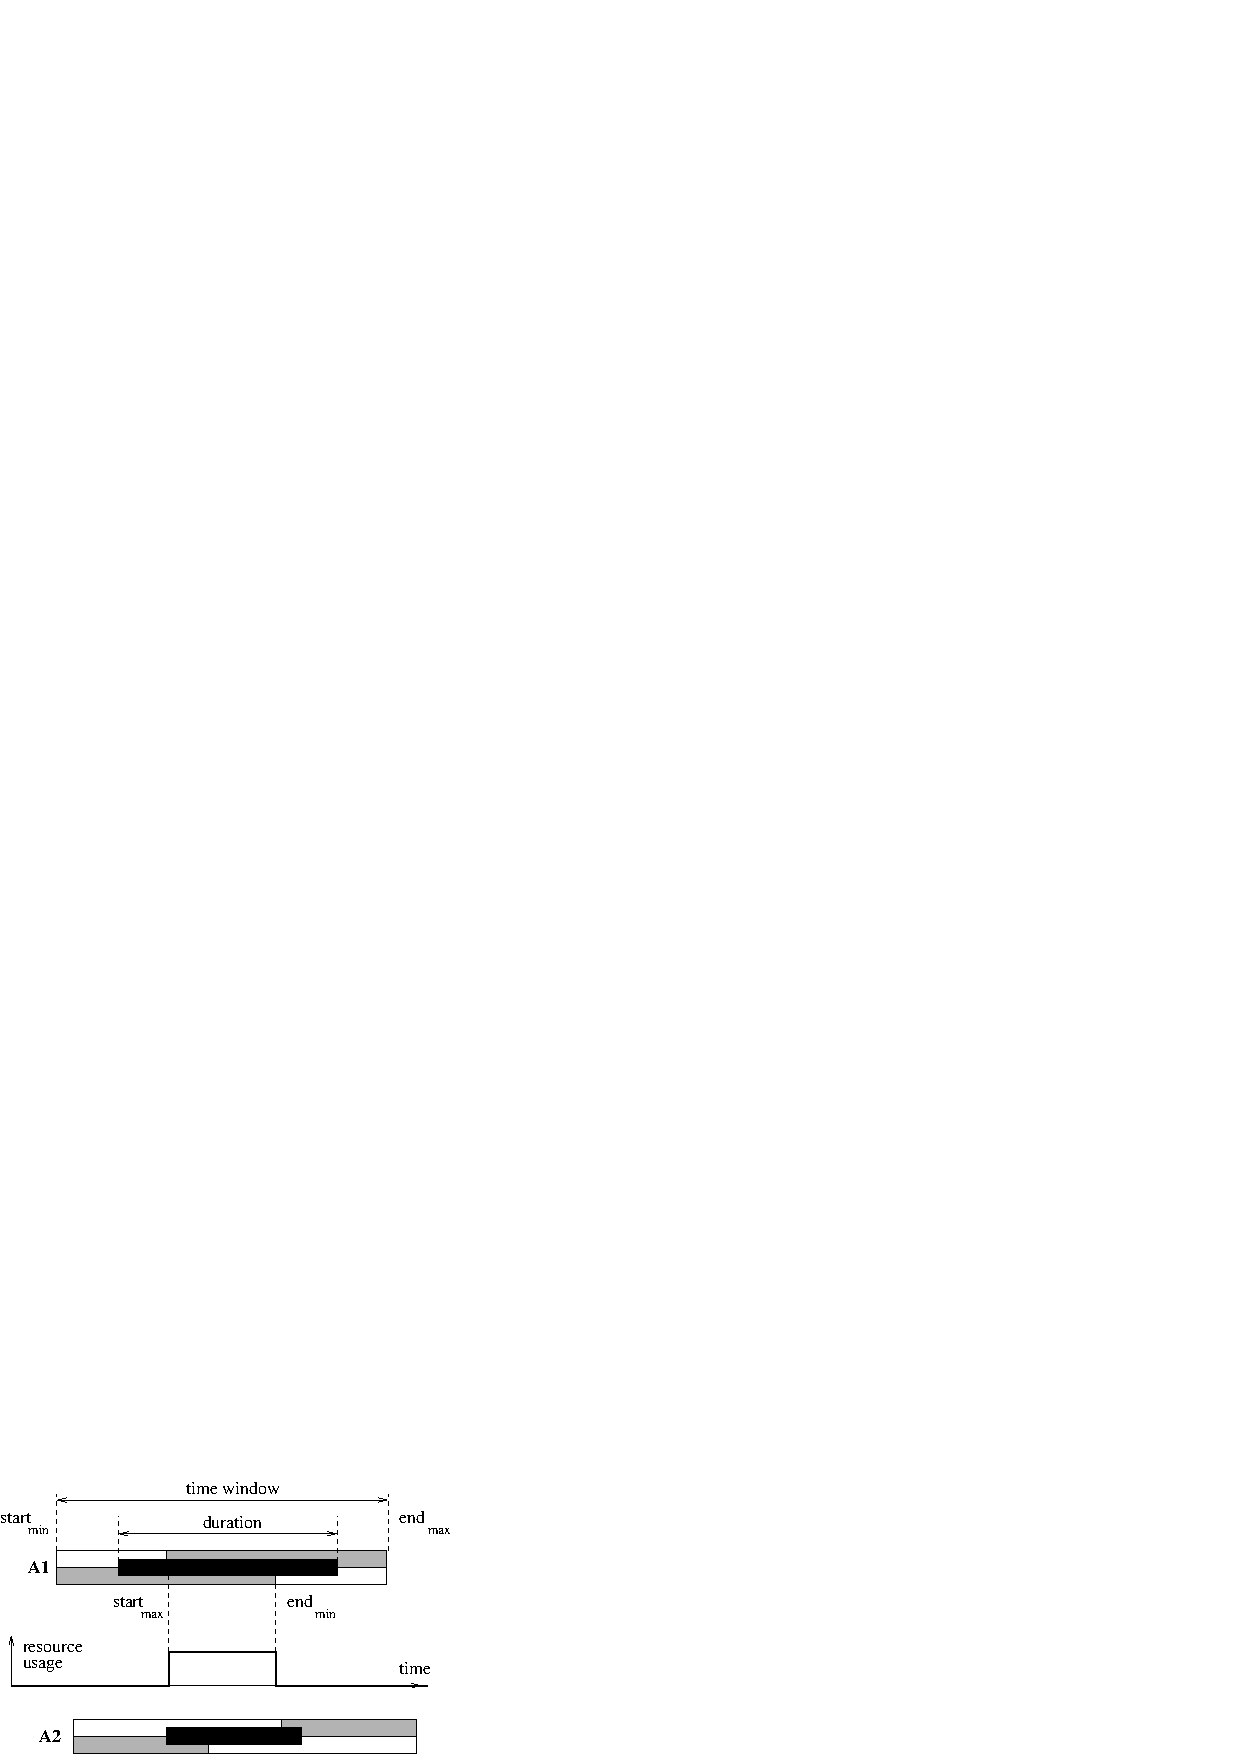
\includegraphics[width=20pc]{figures/fig1.pdf}}
\caption{Limitations of Resource Profiling Approaches}
\label{fig1}
\end{figure}


\subsection{Activity Interactions}

The  second family of  algorithms is based  on an analysis of activity
interactions.  Instead  of considering what happens  at a date $t$, it
considers subsets $\Omega$ of  activities competing for the  same
resource   and  performs propagation  based   on the  position of
activities in $\Omega$. Some classical activity interaction approaches
are summarized below.

\subsubsection{Disjunctive Constraint.}  The  simplest example of such
an algorithm    is  the  disjunctive   constraint on   unary resources
\cite{erschler76}.  This algorithm  analyzes  each pair of  activities
$(A,B)$ requiring the  same unary resource.  Whenever the current time
bounds of activities are such that $start_{max}(A) < end_{min}(B)$, it
deduces that, as  activity $A$  necessarily starts  before the  end of
activity $B$, it must be completely executed before $B$. Thus, $end(A)
\le start_{max}(B)$ and $start(B) \ge end_{min}(A)$.

Actually,  on a unary   resource, the classical disjunctive constraint
can  be generalized as  follows: whenever the temporal constraints are
such     that      the       constraint    $start(A)<end(B)$      must
hold\footnote{$start_{max}(A) <  end_{min}(B)$  is  only  a sufficient
condition for the precedence constraint $start(A)<end(B)$ to hold. The
extended  disjunctive  constraint  allows propagation  even  when this
precedence constraint is  not  a  consequence  of the  time-bounds  of
activities but, for example, belongs   to the initial problem or   has
been added as a decision in the search tree.},  it adds the additional
constraint that $end(A) \le start(B)$. Note that this algorithm is the
exact  counterpart in  scheduling  of  the disjunctive constraint   to
handle    unsafe  causal  links    in    POCL planners    proposed  in
\cite{khambhampati96}.   Unfortunately,  such a simple constraint only
works in the restricted case of unary resources.

\subsubsection{Edge-Finding.}           Edge-finding        techniques
\cite{carlier90,nuijten94}  are  available for both unary (disjunctive
scheduling) and discrete resources (cumulative scheduling). On a unary
resource, edge-finding  techniques  detect situations   where a  given
activity  $A$ cannot execute  after  any  activity  in a  set $\Omega$
because there would  not be enough time to  execute all the activities
in $\Omega \cup  A$ between the  earliest start time  of activities in
$\Omega \cup A$ and the latest end  time of activities in $\Omega \cup
A$.  When such   a situation occurs,  it  means that $A$ must  execute
before all the activities  in $\Omega$ and  it allows computing a  new
valid upper bound for the end time of $A$. More formally, let $\Omega$
be a subset of  activities on a  unary resource, and $A \notin \Omega$
another activity on the  same  unary resource.   If  $start_{min}(X)$,
$end_{max}(X)$  and  $dur_{min}(X)$   respectively denote  the minimal
start time, maximal end time and minimal  duration over all activities
in a set  $X$, most of the edge-finding  techniques can be captured by
the rule $(1) \Rightarrow (2)$ where:

\begin{eqnarray*} 
(1) & end_{max}(\Omega \cup A) - start_{min}(\Omega) < dur_{min}(\Omega \cup A) \\
(2) & end(A) \leq \min_{\Omega' \subseteq \Omega}{(end_{max}(\Omega') - dur_{min}(\Omega'))}
\end{eqnarray*}

In  the example    of Figure \ref{fig2},  if   we   take $A=A_4$   and
$\Omega=\{A_1,A_2,A_3\}$,   we  see    that  the  conditions   of  the
propagation   rule are satisfied as  $end_{max}(\Omega  \cup A) = 16$,
$start_{min}(\Omega)  = 6$   and  $dur(\Omega  \cup  A)   =  11$.  The
edge-finding algorithm would compute a new upper bound on the end time
of   $A_4$     equal      to    $16-9=7$    realized      by    taking
$\Omega'=\{A_1,A_2,A_3\}$.

\begin{figure}
\centerline{\includegraphics[width=28pc]{figures/fig2.pdf}}
\caption{Example of Edge-Finding Propagation}
\label{fig2}
\end{figure}

Similar rules allow us to  detect and propagate  the fact that a given
activity  must  end after  all  activities  in $\Omega$  ({\em Last}),
cannot start before all  activities in $\Omega$  ({\em Not First})  or
cannot end  after  all activities  in $\Omega$ ({\em  Not  Last}). See
\cite{torres00}    for    more   details.   Furthermore,  edge-finding
techniques can be  adapted to discrete  resources by reasoning on  the
resource  energy required  by  the  activities; that  is,  the product
$duration    \times     required~quantity~of~resource$.  Most   of the
edge-finding algorithms can be implemented to propagate on all the $n$
activities and  all the  subsets $\Omega$  with a total  complexity in
$O(n^2)$ \cite{baptiste00}.

\subsubsection{Energetic Reasoning.}  Whereas edge-finding  techniques
compare  the temporal characteristics of an  activity $A$ with respect
to a set of activities $\Omega$, energetic reasoning \cite{erschler91}
consists  in comparing the  amount of resource  energy required over a
time interval   $[t_1,t_2)$  to the  total amount   of energy  that is
available over the same interval.  Both the edge-finding and energetic
reasoning techniques analyze  the current time-bounds of activities in
order to adjust them by removing some invalid values.

A typical example of energetic  reasoning consists in finding pairs of
activities $(A,B)$ on a unary resource such that ordering activity $A$
before $B$ would lead  to a dead  end because the unary resource would
not provide  enough ``energy'' between  the earliest start time of $A$
and the latest end time of  $B$ to execute $A$,  $B$ and all the other
activities that  necessarily   need to  partly  execute  on this  time
window.  More formally,  if $C$ is  an activity and $[t_1,t_2)$ a time
window,  the  energy necessarily required  by $C$  on the  time window
$[t_1,t_2)$ is:

{\setlength\arraycolsep{2pt}
 \begin{eqnarray}
 W_C^{[t_1,t_2)} = \max(\ 0,\ \min(\ & end_{min}(C)-t_1,\ & t_2 - start_{max}(C), \nonumber\\
 &\ dur_{min}(C),\ & t_2 - t_1 \ )\ ) \nonumber
\end{eqnarray}}

Thus, as soon as  the condition below  holds, it means that $A$ cannot
be ordered before $B$ and thus, must be ordered after.
\begin{eqnarray*} 
end_{max}(B) - start_{min}(A) < ~~~~~~~~~~~~~~~~~~~~~~~~~~~~~~~~~~~~~~~\\
dur_{min}(A) + dur_{min}(B) + \sum_{C \notin \{A,B\}}{W_C^{[start_{min}(A), end_{max}(B))} }
\end{eqnarray*}

This rule allows the update of the earliest start time  of $A$ and the
latest end time of $B$.

Other  adjustments of time  bounds using  energetic  reasoning  can be
used, for example,  to  deduce that  an activity cannot  start  at its
earliest start time or cannot end at its latest end time. Furthermore,
energetic reasoning can easily be extended to discrete resources.

A good starting  point to learn more  about edge-finding and energetic
reasoning  are   \cite{baptiste95, dorndorf99,  baptiste00} where  the
authors describe and  compare  several variants of   these techniques.
Although  these  tools (edge-finding,  energetic   reasoning) are very
efficient  in pure  scheduling  problems, they  suffer from  the  same
limitations as  timetabling   techniques.  Because  they  consider the
absolute position   of activities in  time (their  time-bounds) rather
than their  relative   position (the precedence   constraints  between
them), they will not propagate  until  the time windows of  activities
are small enough. The propagation may be very limited when the current
schedule  contains many  precedence constraints.   Furthermore,  these
tools  are  available for unary  and  discrete resources  only and are
difficult to generalize to reservoirs.

The following sections  of this paper  describes two new techniques to
propagate discrete and  reservoir  resources  based on  analyzing  the
relative position of activities rather than their absolute position in
time.   These algorithms exploit   the precedence  constraints between
activities and propagate even when the time  windows of activities are
still  very large  (which is typically   the  case in least-commitment
planners and schedulers). Of course - and this is  one of the strength
of constraint programming  - these new  propagation  algorithms can be
used in  cooperation with  the  existing techniques we just  described
above.   Both of  our  algorithms  are based on  the  precedence graph
structure presented in the next section.

\section{Precedence Graph \label{precgraph}}

\subsection{Definitions} A  resource event $x$ on  a resource $R$ is a
variable time-point at which the  availability of the resource changes
because of an activity.  A resource  event corresponds to the start or
end point of an activity. Let:
\begin{itemize}
\item $t(x)$ denote the variable  date of event $x$. $t_{min}(x)$  and
      $t_{max}(x)$ will   respectively denote the current  minimal and
      maximal value in the domain of $t(x)$.
\item $q(x)$  denote the relative  change of resource availability due
      to event  $x$  with the usual  convention that   $q>0$ denotes a
      resource       production    and        $q<0$     a     resource
      consumption. $q_{min}(x)$  and $q_{max}(x)$  will   respectively
      denote  the current minimal and  maximal values in the domain of
      $q(x)$.
\end{itemize} 

There is of course an evident mapping between the resource constraints
on a resource and the resource events as illustrated in Figure \ref{fig3}.  
Depending  on the  time extent,  a resource constraint is
mapped to one or two resource events.

Note that if the availability of the resource changes over time, dummy
events may be introduced to accommodate  this availability profile. Of
course, these dummy events may impact the complexity.

A  precedence    graph on   a  resource   $R$   is  a  directed  graph
$G_R=(V,E_{\le},E_{<})$ where $E_{<} \subseteq E_{\le}$ and:
\begin{itemize}
\item $V$ is the set of resource events on $R$ 
\item $E_{\le} =\{(x,y)\}$ is the set  of precedence relations between
      events of the form $t(x) \le t(y)$.
\item $E_{<} =\{(x,y)\}$  is  the set of  precedence relations between
      events of the form $t(x) < t(y)$.
\end{itemize}

The precedence graph on  a  resource is designed  to collect  all  the
precedence  information  between  events   on  the  resource.    These
precedence information may come from:  (1) temporal constraints in the
initial statement  of the  problem,  (2) temporal  constraints between
activities  inserted by   the  same  planning  operator, (3)    search
decisions   (e.g.    causal link,   promotion,  demotion  \cite{snlp},
ordering decisions on  resources) or (4)  may have been discovered  by
propagation   algorithms    (e.g.   unsafe   causal   links   handling
\cite{khambhampati96},   disjunctive constraint,   edge-finding,    or
balance  constraint as described   in section \ref{balance}) or simply
because $t_{max}(x) \le t_{min}(y)$. When new events or new precedence
relations  are inserted, the  precedence graph incrementally maintains
its transitive closure
\cite{laborie-00}.  The precedence relations in the precedence graph as
well as  the   initial  temporal  constraints  are  propagated by   an
arc-consistency algorithm.   Given an event  $x$ in a precedence graph
and assuming the transitive closure  has been computed, we define  the
following subsets of events:
\begin{itemize}
\item $S(x)$ is the set  of events simultaneous with  $x$; that is, the
      events $y$ such   that  $(x,y)  \in   E_{\le}$ and  $(y,x)   \in
      E_{\le}$. Note that $x \in S(x)$.
\item $B(x)$ is  the set of events before  $x$; that is, the events $y$
      such that $(y,x) \in E_{<}$
\item $BS(x)$ is  the set of events   before or simultaneous  with $x$;
      that is, the  events $y$ such that  $(y,x) \in  E_{\le}$ , $(y,x)
      \notin E_{<}$ and $(x,y)\notin E_{\le}$
\item $A(x)$ is the  set of events  after $x$;  that is, the  events $y$
      such that $(x,y)\in E_{<}$
\item $AS(x)$ is the set of events after or simultaneous with $x$; that
      is, the  events $y$  such  that $(x,y)\in  E_{\le}$ , $(x,y)
      \notin E_{<}$ and $(y,x)\notin E_{\le}$
\item $U(x)$ is the set of events unranked with respect to $x$; that is,
      the events $y$  such that $(y,x)\notin E_{\le}$ and $(x,y)\notin
      E_{\le}$
\end{itemize}

Note that for any event $x$, $\{S(x), B(x), BS(x), A(x), AS(x),U(x)\}$
is a partition    of $V$.  An   example of  precedence graph with   an
illustration of   these subsets is  given   in Figure  \ref{fig4}.  On
figures depicting precedence  graphs, a solid  arc  between two events
$x$ and  $y$  denotes a constraint   $t(x)<t(y)$ whereas a  dotted arc
denotes a constraint $t(x) \leq t(y)$.  The graph in Figure \ref{fig4}
corresponds  to  a current schedule  with   the 6 resource constraints
listed below and some precedence relations.

\begin{tabular}{lll}
$<A_1,R,-2,FromStartToEnd>$, &$<A_2,R,[-10,-5],AfterStart>$,\\
$<A_3,R,-1,AfterStart>$,     &$<A_4,R,           +4,AfterEnd>$,\\
$<A_5,R,+2,AfterEnd>$,       &$<A_6,R,+2,AfterEnd>$
\end{tabular}

The  subsets in   Figure \ref{fig4} are   relative  to the  event  $x$
corresponding to the start of activity $A_1$.

\begin{figure}
\centerline{\includegraphics[width=20pc]{figures/fig4.pdf}}
\caption{An Example of Precedence Graph}
\label{fig4}
\end{figure}

\subsection{Implementation and Complexity}  As   we will see   in next
section, our propagation algorithms often need to query the precedence
graph about the relative position of two events on a resource, so this
information needs to  be  accessible in $O(1)$.   It explains  why  we
chose to implement the  precedence graph as a  matrix that  stores the
relative  position of   every  pair of events.     Furthermore, in our
structure, the complexity  of traversing any  subset of  events (e.g.,
$B(x)$ or $U(x)$) is equal to  the size of this  subset. Note that the
precedence graph  structure is extensively  used in ILOG Scheduler and
is not  only useful for  the algorithms described  in  this paper.  In
particular,  the precedence graph  implementation  allows the user  to
write his own  complex constraints that rely   on this graph,  as, for
example, the one  involving alternative resources and transition times
described in
\cite{focacci00}.

\section{New Propagation Algorithms}

\subsection{Introduction}

We describe in     this  section  two  new    propagation   algorithms
respectively on  discrete  resources  and reservoirs.    Like previous
propagation  algorithms, both of  them are  used to  discover new time
bounds  and/or new  precedence   relations   on the   current  partial
schedule.   The main originality of  our algorithms relies on the fact
that  they  analyze the  relative position   of activities (precedence
relations in the precedence graph) rather than their absolute position
only as  it was the case   for previous algorithms. As  a consequence,
they  allow a much  stronger   propagation when  the time windows   of
activities is large  and when the  current schedule contains a lot  of
precedence   relations, which is  typically  the case when integrating
planning and scheduling.

\subsection{Energy Precedence Constraint}  

The  energy precedence  constraint is  defined  on  discrete resources
only. It  does not require the  resource to be  closed (new activities
and resource constraint   can be added  later  on in the  search tree)
thus, it can be  used at any time  during the search.  For simplicity,
we  assume that  all  the   resource constraints have  a   time extent
$FromStartToEnd$. Suppose that $Q$ denotes the maximal capacity of the
discrete resource over time.  If $x$  is a resource event and $\Omega$
is a  subset of resource constraints  that are  constrained to execute
before  $x$, then the  resource must provide  enough energy to execute
all resource constraints in  $\Omega$ between the earliest start times
of activities of $\Omega$ and $t(x)$. More formally:
\[t_{min}(x) \ge \min_{<A,R,q>\in \Omega} (start_{min}(A)) +
\frac{\sum_{<A,R,q>\in \Omega} (|q_{max}(A)| \cdot dur_{min}(A))}{Q}\]
A very simple example of  the propagation performed by this constraint
is given in Figure \ref{fig5}. If we suppose that the maximal capacity
of the discrete  resource is $4$ and all  activities must  start after
time $0$, then by considering $\Omega=\{A_1, A_2,  A_3, A_4\}$, we see
that event $x$ cannot  be executed before  time $[0]+[(2 \times 10)+(2
\times 2)+(2 \times 8)+(2 \times 8)]/4 = 14$. Of course, a symmetrical
rule can be used  to find an upper bound  on $t(x)$ by considering the
subsets $\Omega$ of resource constraints that  must execute after $x$.
The same idea as the energy precedence constraint is used in
\cite{sourd00}  to adjust the  time-bounds  of activities on different
unary resources.

\begin{figure}
\centerline{\includegraphics[width=20pc]{figures/fig5.pdf}}
\caption{Example of Energy Precedence Propagation}
\label{fig5}
\end{figure}

It's important to note that the energy precedence algorithm propagates
even when the time window of activities is  very loose (in the example
of Figure \ref{fig5},  the latest end times of  activities may be very
large). This is  an  important difference  with respect   to classical
energetic and edge-finding  techniques that would propagate nothing in
this case.

The propagation of the  energy precedence constraint can be  performed
for all the events $x$ on a resource and  for all the subsets $\Omega$
with a total worst-case time  complexity of $O(n\ (p+log(n))$ where $n$
is the number of the events on the resource and $p$ the maximal number
of predecessors of a given event in the graph ($p < n$).

\subsection{Balance Constraint \label{balance}}

The balance  constraint is  defined  on a   reservoir resource.   When
applied to a  reservoir, the basic version  of this algorithm requires
the reservoir to be closed.  When applied to  a discrete resource, the
resource may still be open.  The basic idea  of the balance constraint
is to compute, for each event $x$ in the precedence graph, a lower and
an upper bound on the reservoir level just  before and just after $x$.
The  reader  will   certainly find  some   similarities   between this
constraint and the Modal Truth  Criterion (MTC) on planning predicates
first introduced in \cite{chapman87}.  Actually this is not surprising
as  the balance constraint   can be considered  as   a kind of MTC  on
reservoirs  that detects  only some necessary  conditions\footnote{One
can   imagine  extending our    propagation   algorithm into   a  real
non-deterministic  ``goal-achievement procedure''  on reservoirs  that
would  allow justifying the  insertion  of new reservoir producers  or
consumers into the current plan when the resource is not closed.  This
extension is  outlined  in  section  \ref{truthcriterion}.}.  Given an
event $x$, using the  graph  we can  compute  an  upper bound  on  the
reservoir level at   date  $t(x)-\epsilon$\footnote{Remember  that  we
assume  that changes of resource  availability only  occur at discrete
times (a time value is an  integer). In this  context one can think of
$\epsilon$ as any  real number in the  interval $(0,1)$.} just  before
$x$ assuming:
\begin{itemize}
\item All   the production  events $y$   that   {\em may} be  executed
      strictly before $x$ are executed strictly before $x$ and produce
      as much as possible; that is, $q_{max}(y)$;
\item All  the consumption events $y$  that {\em need}  to be executed
      strictly before $x$ are executed strictly before $x$ and consume
      as  little  as  possible;  that is,  $q_{max}(y)$\footnote{For a
      consumption event,  $q<0$ and thus, $q_{max}$ really corresponds
      to the smallest consumption of the event.}; and
\item All the consumption events that {\em may} execute simultaneously
      or after $x$ are executed simultaneously or after $x$.
\end{itemize}

For simplicity we assume in this paper that the reservoir is initially
empty (initial level equal to  zero). If this is not  the case, we can
always add a  producing event that  produces the initial level of  the
reservoir at the time origin of the schedule.

More formally, if $P$ is the set of  production events and $C$ the set
of consumption events, this upper bound can be computed as follows:

\begin{eqnarray}
\label{formula1}
L^{<}_{max}(x) = \hspace{-5mm} \sum_{y \in P \cap (B(x) \cup BS(x) \cup
U(x))} \hspace{-14mm} q_{max}(y) + \sum_{y \in C \cap B(x)} \hspace{-4mm} q_{max}(y)
\end{eqnarray}

Applying   this formula to  event $x$ in  Figure \ref{fig4} leads to
$L^{<}_{max}(x)= (+4+2+2) + (-5) =3$.

In  case  of a     consuming  resource constraint   of time     extent
$FromStartToEnd$, and if both the start  and end event of the resource
constraint are  in $BS(x) \cup U(x)$,  it is important to  notice that
those two opposite events can be ignored by the balance constraint for
the computation of  $L^{<}_{max}(x)$.  Indeed, any attempt to  execute
the  production event (end event) before  $x$ would also constrain the
opposite consumption event (start event) to be executed before $x$ and
the global contribution of the resource constraint would then be equal
to zero.  This adjustment is very  important for discrete resources as
most of the resource constraints  on  discrete resource are  precisely
consuming     resource          constraints   of        time    extent
$FromStartToEnd$. Although  this adjustment  of the balance constraint
was implemented, for simplicity, we do not take it into account in the
rest of this article.

In a very similar way, it is possible to compute:
\begin{itemize}
\item $L^{<}_{min}(x)$: a lower bound of the level just before $x$
\item $L^{>}_{max}(x)$: an upper bound of the level just after $x$
\item $L^{>}_{min}(x)$: a lower bound of the level just after $x$
\end{itemize} 

For each of these  bounds, the balance constraint  is able to discover
four types of  information: dead ends, new  bounds for  resource usage
variables,  new  bounds  for   time   variables,  and  new  precedence
relations.  For  symmetry  reasons, we describe only   the propagation
based on $L^{<}_{max}(x)$.

\subsubsection{Discovering  dead  ends.}   This  is the  most  trivial
propagation: whenever $L^{<}_{max}(x)<0$,  we  know that the  level of
the reservoir  will surely be negative  just  before event $x$  so the
search has reached a dead end.

\subsubsection{Discovering new bounds  on  resource usage  variables.}
Suppose  there   exists  a consumption  event $y\in    B(x)$ such that
$q_{max}(y)-q_{min}(y)>L^{<}_{max}(x)$.     If  $y$  would  consume  a
quantity $q$  such that $q_{max}(y)-q>L^{<}_{max}(x)$  then, simply by
replacing $q_{max}(y)$ by $q(y)$ in formula (1), we see that the level
of the reservoir would be negative just before  $x$. Thus, we can find
a     better    lower      bound       on      $q(y)$     equal     to
$q_{max}(y)-L^{<}_{max}(x)$. In the example of Figure \ref{fig4}, this
propagation would restrict  the consumed quantity  at the beginning of
activity $A_2$ to $[-8,-5]$ as any value lower than $-8$ would lead to
a dead end. Similar reasoning  can be applied  to production events in
$B(x) \cup BS(x) \cup U(x)$.

\subsubsection{Discovering   new    bounds    on      time  variables.
\label{newbounds}} Formula (\ref{formula1}) can be rewritten as follows:

\begin{eqnarray}
\label{formula2}
L^{<}_{max}(x) = \hspace{-2mm} \sum_{y \in B(x)} \hspace{-2mm}
q_{max}(y) +  \hspace{-5mm}\sum_{y \in P \cap (BS(x) \cup U(x))}
\hspace{-10mm} q_{max}(y)
\end{eqnarray}

If the first term of  this equation  is  negative, it means that  some
production  events  in  $BS(x) \cup   U(x)$ will have  to be  executed
strictly before $x$ in order to produce at least:

\begin{eqnarray*}
\Pi^{<}_{min}(x) = - \sum_{y \in B(x)}\hspace{-2mm} q_{max}(y)
\end{eqnarray*}

Let  $P(x)$ denote  the   set of   production  events in   $BS(x) \cup
U(x)$. We suppose the  events $(y_1,\cdots,y_i,\cdots,y_p)$  in $P(x)$
are  ordered by increasing minimal time  $t_{min}(y)$. Let  $k$ be the
index in $[1,p]$ such that:

\begin{eqnarray*}
\sum_{i=1}^{k-1}q_{max}(y_i) < \Pi^{<}_{min}(x) \le \sum_{i=1}^{k}q_{max}(y_i)
\end{eqnarray*}

If event $x$ is executed at a date $t(x) \le t_{min}(y_k)$, not enough
producers will be   able to execute  strictly  before $x$  in order to
ensure  a positive level just before  $x$. Thus, $t_{min}(y_k)+1$ is a
valid lower bound of $t(x)$. In Figure \ref{fig4},
$\Pi^{<}_{min}(x)=5$, and  this propagation  will  deduce that  $t(x)$
must be  strictly greater  than the  minimal between the  earliest end
time of $A_5$ and the earliest end time of $A_6$.

\subsubsection{Discovering new  precedence relations.\label{dnpr}} There are cases
where we can perform an even stronger  propagation.  Let $P(x)$ denote
the  set  of production  events  in $BS(x)  \cup  U(x)$. Suppose there
exists a production event $y$ in $P(x)$ such that:
\begin{eqnarray*}
\sum_{z \in P(x) \cap (B(y) \cup BS(y) \cup U(y))} \hspace{-14mm}
q_{max}(z) < \Pi^{<}_{min}(x) 
\end{eqnarray*}

Then, if we  had $t(x)\le t(y)$,  we would see  that again there is no
way to produce $\Pi^{<}_{min}(x)$ before  event $x$ as the only events
that  could produce strictly  before event $x$ are  the  ones in $P(x)
\cap (B(y) \cup BS(y) \cup U(y))$.   Thus, we can deduce the necessary
precedence relation:  $t(y)<t(x)$.  For example  on Figure \ref{fig4},
the balance  algorithm  would discover that $x$  needs  to be executed
strictly  after the end  of $A_4$. Note that  a weaker version of this
propagation has been proposed in  \cite{cesta97} that runs in $O(n^2)$
and does  not analyze the precedence relations  between the  events of
$P(x)$.

Note also   that the precedence  relations  discovered by  the balance
constraint can be rephrased in terms of algorithms on Minimal Critical
Sets (MCSs) \cite{laborie95}. On a discrete resource, a MCS is defined
as a minimal set  of activities (for  the set inclusion) such that all
the activities  in  the  set may  globally  overlap  and  the combined
capacity requirement is greater than the  resource capacity.  MCSs can
be  generalized on reservoirs by    transforming the reservoir into  a
discrete resource as follows.  Any consumption event $x$ is considered
as a   requirement of  a  quantity  $|q(x)|$  over  the time  interval
$[t(x),+\infty)$ and any  production event $y$ as  a  requirement of a
quantity $|q(y)|$   over the time interval  $[-  \infty,  t(y))$.  The
capacity of the discrete resource is equal to  the maximal capacity of
the reservoir plus the sum of the quantities $q(y)$ of each production
event.  Given  an  MCS $\Phi=\{A_1,\cdots,A_n\}$, it  is sufficient to
post one of the precedence relations $A_i  \preceq A_j$ between a pair
of activities in the MCS  to solve the potential  conflict.  An MCS is
said to be deterministic if all those precedence relations but one are
incoherent  with the current   temporal network.   In  this case,  the
unique coherent precedence  relation   can be inferred  by  constraint
propagation   without opening a  choice  point.  The problem with this
approach is that the  number of MCS grows  exponentially with the size
of the problem. In this context, the balance constraint can be seen as
an  algorithm that  implicitly detects and   solves some deterministic
MCSs on the reservoir - as each  precedence relation discovered by the
algorithm necessarily belongs to at least one MCS - while avoiding the
combinatorial explosion of enumerating these MCSs.

\subsubsection{Balance constraint properties  \label{balanceprop}} One
can show that the balance algorithm - like timetabling approaches - is
sound that is, it  will detect a dead  end  on any fully  instantiated
schedule that  violates the reservoir  resource constraint.   In fact,
the  balance algorithm  does  not even need   the schedule to be fully
instantiated: for    example,  it will detect   a   dead  end  on  any
non-solution schedule as soon as all the production events are ordered
relatively to all the consumption events on each resource.

We say that an event $x$ is {\em safe} if and only if $x$ is such that
$L^{<}_{max}(x)\le Q$,  $L^{>}_{max}(x) \le Q$, $L^{<}_{min}(x)\ge 0$,
and $L^{>}_{min}(x)\ge 0$.  It is easy to see that when all events $x$
on a reservoir are safe, any instantiation consistent with the current
precedence graph satisfies  the reservoir constraint.  In other words,
the  reservoir is solved.   This very important  property allows us to
stop the search on a reservoir when  all the events  are safe and even
if they are  not completely ordered.  Note anyway  that the  fact that
all  events are safe   is only a   sufficient condition for  a partial
schedule to be   a  solution.  Because  the  bounds  $L^{<}_{min}(x)$,
$L^{>}_{min}(x)$,  $L^{<}_{max}(x)$ and  $L^{>}_{max}(x)$, are not the
tightest lower and upper bounds on the reservoir level, this criterion
is not a necessary condition. Thus,  relying on this criterion to stop
the search may still lead to  unnecessarily constrained solutions.  We
will see in section \ref{orderk} how to improve the tightness of these
bounds.

The balance algorithm  can   be executed  for all  the  events on  the
reservoir  with a  global worst-case   complexity  in $O(n^2)$  if the
propagation that discovers new  precedence relations is not turned on,
in $O(n^3)$ for a full propagation.   In practice, there are many ways
to shortcut this  worst case and  in  particular, we noticed that  the
algorithmic  cost    of  the   extra-propagation that   discovers  new
precedence  relations was negligible.   In our implementation, at each
node of the  search,  the  full  balance constraint  is executed  from
scratch\footnote{More   precisely,   as   mentioned    in      section
\ref{precgraph}, the sets $S(x)$, $B(x)$, $A(x)$, $BS(x)$, $AS(x)$ and
$U(x)$ are maintained incrementally in the precedence graph.  Only the
levels   $L^{<}_{max}(x)$,  $L^{>}_{max}(x)$,   $L^{<}_{min}(x)$,  and
$L^{>}_{min}(x)$ are  recomputed from scratch.} until a fixed point is
reached.

\subsection{Comparison}

Both the energy precedence and  the balance algorithms can be  applied
to  discrete resources   and rely  on  an  analyze of  the  precedence
relations between activities.  An  interesting question is how the two
propagation techniques perform relative to one another. In fact, it is
easy to see that no one technique dominate the other and that they are
complementary.  The  energy  precedence   propagation relies  on  some
global  {\em energetical}  considerations, as such,   it is closer  to
edge-finding and energetical reasoning whereas the balance propagation
reasons on the  {\em level} of the  resource  and, from this point  of
view, is closer to  timetabling approaches.  Because  it does not take
the duration of activities into account, the balance constraint is for
instance not able to propagate in the case of  figure \ref{fig5}.  The
energy precedence algorithm does not discover new relative positioning
of events and for instance  on the configuration of figure \ref{fig19}
on a discrete resource of maximal capacity  $2$, it would not discover
that          activity     $A_3$        must          start      after
$\min(end_{min}(A_1),end_{min}(A_2))$.   This adjustment  is found  by
the balance constraint.

\begin{figure}
\centerline{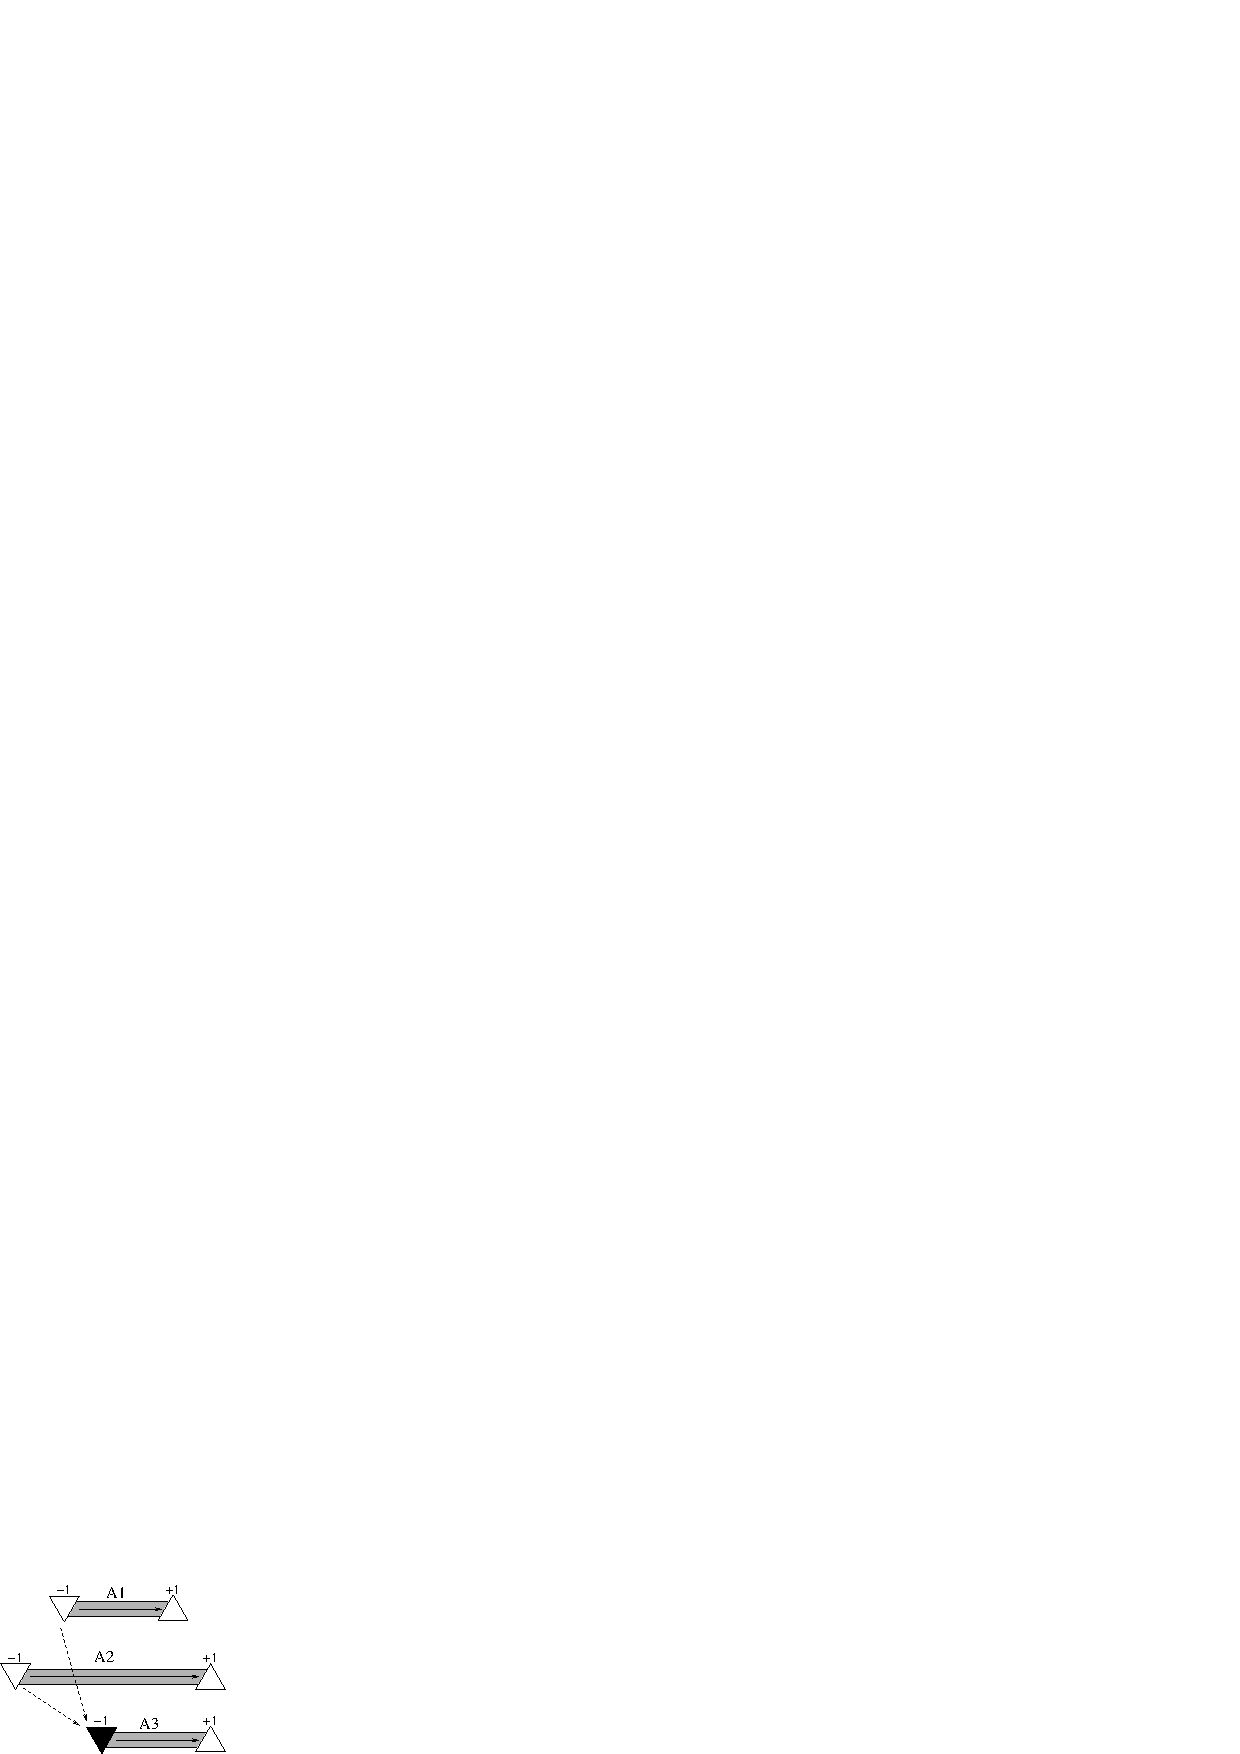
\includegraphics[width=12pc]{figures/fig19.pdf}}
\caption{Propagation of the balance constraint on a discrete resource}
\label{fig19}
\end{figure}

So  one can expect the  precedence energy to  be  effective as soon as
there   are some precedence     constraints  of the  form  $end(A)\leq
start(B)$ between  activities   on the discrete resource   whereas the
balance constraint  will  be more  effective  in presence  of temporal
constraints  of the   form  $start(A) \leq  start(B)$,  $start(A) \leq
end(B)$ or $end(A) \leq end(B)$.

\section{Search}

Before we  describe in detail a  search procedure and heuristics based
on the balance constraint for pure scheduling problems, the subsection
below introduces some basic blocks used by the search.

\subsection{Basic blocks \label{basics}}

\subsubsection{Reservoir levels.\label{reslevels}}

Let   $x$  be  an    event  on   a  reservoir  of   capacity   $Q$ and
$L^{<}_{max}(x)$,    $L^{>}_{max}(x)$,       $L^{<}_{min}(x)$,     and
$L^{>}_{min}(x)$ the levels computed  by   the balance constraint   as
described in section \ref{balance}.

We can define the following quantities:
\begin{itemize}
\item $lack^<(x) = max (0, -L^{<}_{min}(x))$  denotes the maximal lack
      of  reservoir just before  event   $x$ estimated by the  balance
      constraint
\item $lack^>(x) = max  (0, -L^{>}_{min}(x))$ denotes the maximal lack
      of reservoir  just after   event  $x$ estimated  by the  balance
      constraint
\item $lack(x) = max (lack^<(x), lack^>(x))$  denotes the maximal lack
      of reservoir  just before  or after event  $x$  estimated by the
      balance constraint
\item $excs^<(x) = max  (0, L^{<}_{max}(x) -  Q)$ denotes  the maximal
      excess  of  reservoir just before   event  $x$ estimated  by the
      balance constraint
\item $excs^>(x) = max  (0, L^{>}_{max}(x) -  Q)$ denotes the  maximal
      excess of reservoir  just after   event  $x$  estimated by   the
      balance constraint
\item $excs(x)   = max   (excs^<(x), excs^>(x))$  denotes  the maximal
      excess of reservoir just before or  after event $x$ estimated by
      the balance constraint
\item if    we   roughly suppose  that       all the  levels   between
      $L^{<}_{min}(x)$       and     $L^{<}_{max}(x)$    and   between
      $L^{>}_{min}(x)$    and      $L^{>}_{max}(x)$  are equiprobable,
      \[prod(x)    =  \frac{L^{>}_{min}(x)    +   L^{>}_{max}(x)     -
      L^{<}_{min}(x) -  L^{<}_{max}(x)}{2}\] estimates  the    average
      reservoir production at the time when event $x$ occurs.
\end{itemize}

Event $x$ will be said  to be a {\em globally  producing} event if and
only  if  $prod(x)>0$; in that  case,  we will  denote it $isProd(x)$;
otherwise, if $prod(x)\leq 0$, we will say that $x$ is a {\em globally
consuming} event and denote it $isCons(x)$.

Event $x$ is  said to be a {\em   globally underflowing} event if  and
only    if    $lack(x)>excs(x)$; in  that    case,    we  will  denote
$isLack(x)$. This means that if we roughly suppose that all the levels
between  $L^{<}_{min}(x)$     and      $L^{<}_{max}(x)$   and  between
$L^{>}_{min}(x)$ and $L^{>}_{max}(x)$ are equiprobable, there are more
chances that the reservoir will underflow  at date $t(x)$ than chances
it  will overflow. Otherwise,  if  $lack(x) \leq  excs(x)$ we will say
that $x$  is a  {\em     globally overflowing}  event and denote    it
$isExcs(x)$. These notions are depicted in Figure \ref{fig8}.

\begin{figure}
\centerline{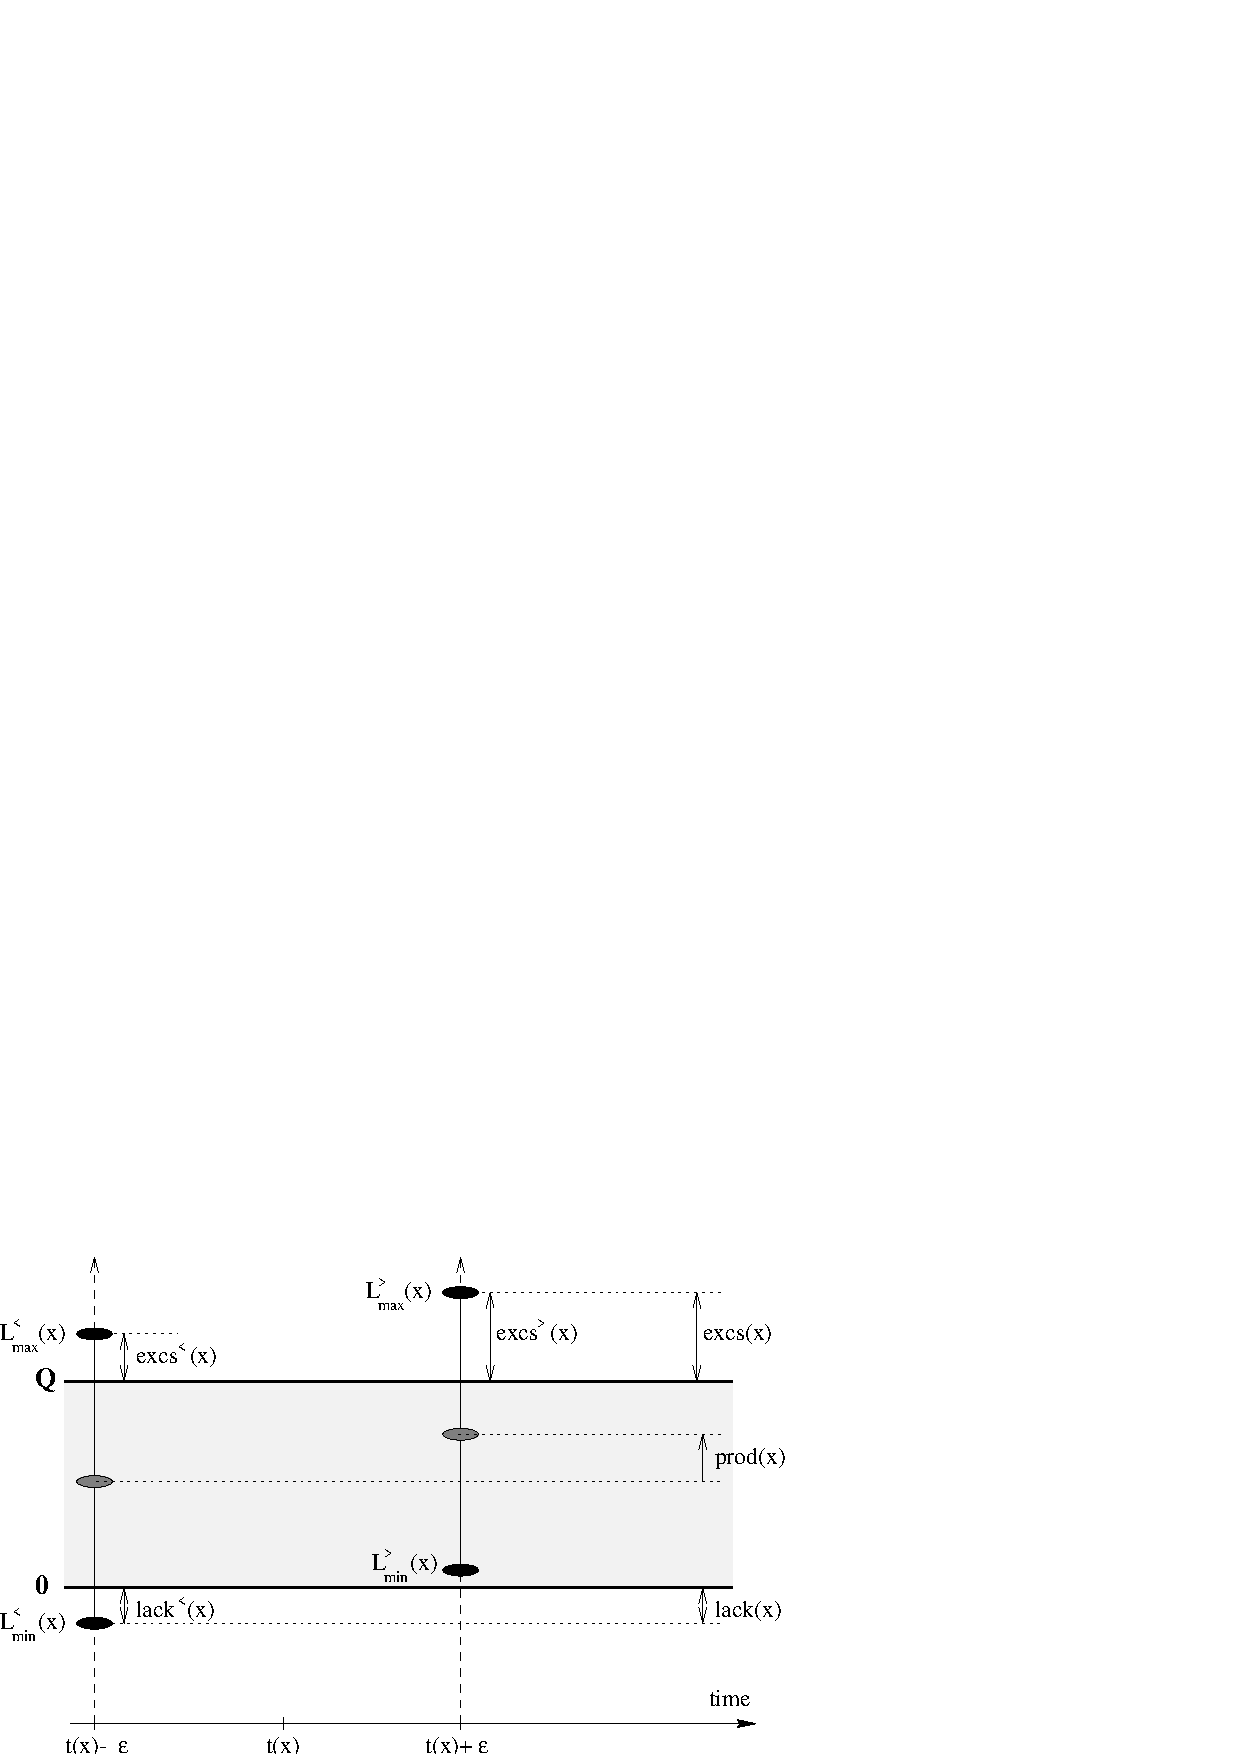
\includegraphics[width=25pc]{figures/fig8.pdf}}
\caption{Reservoir levels}
\label{fig8}
\end{figure}

\subsubsection{Temporal commitment.\label{tempcommit}}

The level of commitment of posting a  constraint is usually defined as
the ratio of fully  grounded  schedules that  are invalidated by  this
constraint.  We describe in this section an estimation of the level of
commitment of posting precedence  constraints between events.  Let $x$
and $y$ be two events  with respective lower  and upper bound for time
value:  $t_{min}(x)$,  $t_{max}(x)$, $t_{min}(y)$,  $t_{max}(y)$.  The
level of  commitment of posting  the constraint $t(x)\leq t(y)$ can be
estimated  as  the ratio of  the  area of the  rectangle $t_{min}(x)$,
$t_{max}(x)$, $t_{min}(y)$, $t_{max}(y)$  that is  invalidated by  the
constraint as  illustrated in Figure \ref{fig9}.  Let $\delta_{min}=1$
if $t_{min}(x)>t_{min}(y)$ and  $0$ otherwise and let $\delta_{max}=1$
if $t_{max}(x)>t_{max}(y)$ and $0$ otherwise. Furthermore, let:

\[ A =  (t_{max}(y) - t_{min}(y)+1) \cdot (t_{max}(x) - t_{min}(x)+1)\]

\[ B = \frac {(t_{max}(x) - t_{min}(y)+1)^2}{2} \]

\[ C_{min} = \frac {(t_{min}(x)-t_{min}(y))^2}{2} \]

\[ C_{max} = \frac {(t_{max}(x)-t_{max}(y))^2}{2} \]

The ratio is then equal to: \small

\[ commit(t(x) \leq t(y)) = \frac  {B - (\delta_{min} \cdot C_{min}) -
(\delta_{max} \cdot C_{max})}{ A }\] \normalsize

\begin{figure}
\centerline{\includegraphics[width=15pc]{figures/fig9.pdf}}
\caption{Temporal commitment}
\label{fig9}
\end{figure}

If temporal constraints are propagated by a path-consistency algorithm
that maintains    the    distances  between   each   pair of    events
$d(x,y)=t(y)-t(x) \in [d_{min},d_{max}]$  then, a better estimation of
the   level of  commitment   of posting $t(x)\leq   t(y)$  is given by
\cite{laborie95}       as:     \[   commit(t(x)      \leq   t(y))    =
\frac{\min(d_{max},0)-\min(d_{min},0)}{d_{max}-d_{min}+1} \]

We can  estimate in the  same way the  level of commitment  of posting
$t(x)<t(y)$ as $commit(t(x)<t(y))=commit(t(x) \leq t(y)-1)$

\subsection{Search procedure overview}

The search procedure works as follows:
\begin{enumerate}
\item select  a      critical    unsafe   event\footnote{C.f.  section
      \ref{balanceprop} for a definition of a safe event.} $x$
\item select a critical unsafe event $y$ unranked with respect to $x$
\item depending    on  the pair   of   events  $(x,y)$,  branch on the
      constraints:
	\begin{itemize}
	\item $t(x) \leq t(y)$ or $t(x) > t(y)$
	\item $t(x) < t(y)$ or $t(x) \geq t(y)$
	\item $t(y) \leq t(x)$ or $t(y) > t(x)$
	\item $t(y) < t(x)$ or $t(y) \geq t(x)$
	\end{itemize} 	
\end{enumerate}

Several search procedures  were     designed depending  on    the  two
criticality evaluation functions: (1) criticality of an event $x$  and
(2) criticality of an    event $y$ to  be   ordered  with respect   to 
$x$.    These     different criticality  evaluations    are  described
below. They all rely on the upper and lower bounds on reservoir levels
$L^{<}_{max}(x)$,       $L^{>}_{max}(x)$,  $L^{<}_{min}(x)$,       and
$L^{>}_{min}(x)$ computed by the  balance constraint. These levels can
indeed  be considered as  some kind of texture measurements\footnote{A
texture is  a  data structure   that maintains  some data useful   for
computing heuristics.}  projected  on the  schedule events.  Actually,
and this is   a very interesting  perspective from   the standpoint of
heuristics, most of the literature on textures, see for example
\cite{beck99}, could be extended and handled at the level of events in
the precedence graph rather than on the absolute time axis.

\subsection{Criticality of an event}

The basic idea is that  an event $x$ is  highly critical if one of its
values  $lack(x)$  or  $excs(x)$  is ``large''  as it   means that the
reservoir may  underflow   or overflow a lot    when $x$ is  executed.
Furthermore, if the temporal  domain $[t_{min}(x),t_{max}(x)]$  of $x$
is small, it means that  there will not be much  room to choose a date
when to execute $x$ and thus, it increases its criticality. Let:
\[t_{\Delta}(x)=1 + t_{max}(x) - t_{min}(x)\]
\[crit^<(x) = \frac{\max(lack^<(x), excs^<(x))}{L^<_{max}(x)-L^<_{min}(x)}\]
\[crit^>(x) = \frac{\max(lack^>(x), excs^>(x))}{L^>_{max}(x)-L^>_{min}(x)}\]

We used three criticality evaluations that implement this idea;
they are defined as follows:

\[crit_1(x) = \frac{\max(crit^<(x), crit^>(x))}{t_{\Delta}(x)}\]
\[crit_2(x) = \frac{\max(lack(x), excs(x))}{Q \cdot t_{\Delta}(x)}\]
\[crit_3(x) = \frac{\max(crit^<(x), crit^>(x))^2}{t_{\Delta}(x)}\]

Note that evaluation $crit_2$ is normalized by the maximal capacity of
the reservoir  and evaluation $crit_3$  gives a higher priority to the
reservoir levels compared to the temporal slack.

\subsection{Criticality of an ordering}

Now suppose that an unsafe event $x$ has been selected by using one of
the three criticality functions described in the previous subsection.

Basically, when an  event $x$ has been selected,  it falls into one of
two categories: either   $x$  is a  globally underflowing  event  or a
globally overflowing event (see section \ref{reslevels}).

Suppose  $x$ is a globally underflowing  and producing event. It means
that   the balance  constraint  estimates   that  there are risks   of
reservoir underflow  at the time  event  $x$ is  executed, and that on
average, the   level  of  the  reservoir  will  be increased   at this
date. Thus, the risk of  underflow is even stronger at $t(x)-\epsilon$
than at $t(x)+\epsilon$.  To fix this  risk of reservoir underflow  at
date $t(x)-\epsilon$,  we can either select a  producing event $y$ and
try   first  posting  the constraint   that $t(y)<t(x)$   or select  a
consuming event $y$ and try  first postponing it  after $x$ by posting
the  constraint $t(x) \leq t(y)$.   Following this idea, the branching
schemes for the possible combinations of  status of events $x$ and $y$
are summarized in the table below.
 
\scriptsize

\begin{center}
\begin{tabular}{|ll|l|l|}\hline
            &              & $isProd(y)$         & $isCons(y)$
            \\ \hline \hline
$isLack(x)$ &  $isProd(x)$ & try $t(y)<t(x)$, then $t(y) \geq t(x)$  & try $t(x) \leq t(y)$, then $t(x) > t(y)$ \\ \hline
$isLack(x)$ &  $isCons(x)$ & try $t(y) \leq t(x)$, then $t(y)>t(x)$  & try $t(x)<t(y)$, then $t(x) \geq t(y)$
\\ \hline \hline
$isExcs(x)$ &  $isProd(x)$ & try $t(x)<t(y)$, then $t(x) \geq t(y)$  & try $t(y) \leq t(x)$, then $t(y) > t(x)$ \\ \hline
$isExcs(x)$ &  $isCons(x)$ & try $t(x) \leq t(y)$, then $t(x)>t(y)$  & try $t(y)<t(x)$, then $t(y) \geq t(x)$ \\ \hline
\end{tabular}
\end{center}

\normalsize

We see that for a pair  of events $(x,y)$  the branching scheme always
looks like {\em try $Ct(x,y)$, then $\neg Ct(x,y)$} where $Ct(x,y)$ is
a precedence  constraint between the two  events. The actual $Ct(x,y)$
depends  on   the status (is   globally  under-  or  overflowing,  is
producing or consuming) of events $x$ and $y$ as shown in the table.

In our search procedure, given $x$, we used three possible evaluations
of event $y$ and select the event $y$ that maximizes this evaluation.

\[crit_a(x,y) = \min(commit(Ct(x,y)),commit(\neg Ct(x,y))) \cdot |prod(y)|\]

\[crit_b(x,y) = commit(Ct(x,y)) \cdot |prod(y)|\]

\[crit_c(x,y) = - \frac{commit(Ct(x,y))}{|prod(y)|}\]

Note  that  $crit_a$ and  $crit_b$ correspond  to   a {\em first fail}
strategy  whereas  $crit_c$ corresponds  to  a {\em  least commitment}
strategy.  Note also that  these criticality measurements are weighted
by  the   estimated  production   (or    consumption)  of  event  $y$:
$|prod(y)|$.

Whenever an event $y$ has been selected  to be ordered with respect to
an event $x$, the  ordering $Ct(x,y)$ is posted  on the left branch of
the  search tree. In  case  of failure,   the opposite  ordering $\neg
Ct(x,y)$ is posted on the  right branch and  search continues until all
the  events are  safe.  This search   procedure is clearly  sound  and
complete.

\section{Results}

\subsection{Balance Constraint}

Until  now, very  few   benchmarks have  been available   for problems
involving  temporal    constraints    and   complex  resources    like
reservoirs. The only one we are aware of is \cite{neumann99} where the
authors  generate    300 project   scheduling  problems   involving  5
reservoirs, min/max  delays between  activities  and  minimization  of
makespan.  From  these 300 problems,  12  hard instances could not  be
solved to  optimality    by their approach.    We   tested the  search
procedure   described  in  the  previous   section  on these  12  open
problems.  All  the other    problems were easily   solved  using  our
approach. The results are summarized in the table below.

\scriptsize
\vspace*{2mm}
\begin{center}
\begin{tabular}{|c|c|c|c|c|c|c|c|}\hline
{\bf $~$Problem$~$} & {\bf $~$Size$~$} &  {LB} & {UB} & {\bf {\it
$~$Opt$~$}} & {\bf {\it $~$Opt$~$}} & {\bf $~$Optimal$~$} & {\bf $~$CPU$~$} \\ 
 & &  &  & {\bf {\it $~$Proof$~$}} & {\bf {\it $~$Sol$~$}} & & {\bf $~$Time (s)$~$} \\ \hline

\#10 &  50 & {\it 92}  & {\it 93}        & 1,a & 3,b & 92 & 0.28 \\ \hline
\#27 &  50 & {\it 85}  & {\it $+\infty$} & 1,b* & 2,a & 96 & 2.43 \\ \hline
\#82 &  50 & {\it 148} & {\it $+\infty$} & 1,a &     & no solution & 0.05\\ \hline
\#6  & 100 & {\it 203} & {\it 223}       & 3,c & 2,a & 211 & 0.97\\ \hline
\#12 & 100 & {\it 192} & {\it 197}       & 1,a & 2,a & 197 & 0.72\\ \hline
\#20 & 100 & {\it 199} & {\it 217}       & 1,a & 1,b & 199 & 0.46\\ \hline
\#30 & 100 & {\it 196} & {\it 218}       & 3,b* & 3,c* & 204 & 2.11\\ \hline
\#41 & 100 & {\it 330} & {\it 364}       & 1,a & 3,b & 337 & 0.62\\ \hline
\#43 & 100 & {\it 283} & {\it $+\infty$} & 2,b* &     & no solution & 7.65\\ \hline
\#54 & 100 & {\it 344} & {\it 360}       & 1,a & 1,b & 344 & 0.46\\ \hline
\#58 & 100 & {\it 317} & {\it 326}       & 1,a & 2,a & 317 & 0.49\\ \hline
\#69 & 100 & {\it 335} & {\it $+\infty$} & 2,c* &     & no solution & 1.96\\ \hline
\end{tabular}
\end{center}
\normalsize

The size of the problem is the number of activities. LB and UB are the
best   lower and upper bounds  of   \cite{neumann99}.  The column {\em
OptSol} describes the  pair $(i,u)$ of  criticality  functions used by
the  search procedure to find  the best solution   that is, a solution
with a  makespan  less than or   equal to the  optimal makespan.   The
column   {\em  OptProof} describes the   pair   $(i,u)$ of criticality
functions  used by the search  procedure for the  proof of optimality;
that is, proving that no solution exists with a makespan strictly less
than the optimal makespan.   The column {\em  CPU Time} is the  sum of
the CPU time to  find the optimal  solution and the  CPU time to prove
the optimality of this   solution using the search control  parameters
described  in the two previous  columns.  This time was  measured on a
HP-UX 9000/785 workstation.   We can  see that all    of the 12   open
problems   have    been   closed  in   less   than  10    seconds  CPU
time. Furthermore, our  approach produces highly parallel schedules as
the balance constraint   implements some sufficient conditions  for  a
partial order between events to be  a solution. For example, the Hasse
diagram  of  the partial  order between activities  corresponding to a
part of  the optimal   solution to  problem  \#41 is  given in  Figure
\ref{fig12}.

For solving these problems, we used the conjunction of the balance and
the  timetable constraint on each   reservoir.   Although it does  not
propagate   more  than the balance   constraint,   we noticed that, in
general,  at each node  the timetable  constraint  (which has a  lower
algorithmic complexity)  helps   the balance constraint to   reach the
fixed point  more quickly.  It  results  in decreasing the propagation
time.  Precedence  constraints are  propagated  by an  arc-consistency
algorithm except for the instances marked with a star (*) in the table
for   which we used a limited   version  of path-consistency to detect
cycles    in    temporal   constraints\footnote{Note    that  the time
performances of  these  instances could be  improved  by using a  more
efficient  algorithm for  cycle detection   as   the one proposed   in
\cite{cesta96}.}.

Figures \ref{fig10} and \ref{fig11}  give a more  precise idea of  how
the  different heuristics behave  on these problems. In these figures,
the 9  search heuristics are compared using  a time  limit of 2mn. One
can notice that  for easy instances, there  is not a large  difference
between heuristics.  But on harder ones, like \#30 or \#27, variations
are greater. Note that all the 9 heuristics allow closing all problems
but problem \#30  in less than 2mn CPU  time.  This  suggests that our
approach is fairly robust.

\begin{figure}
\centerline{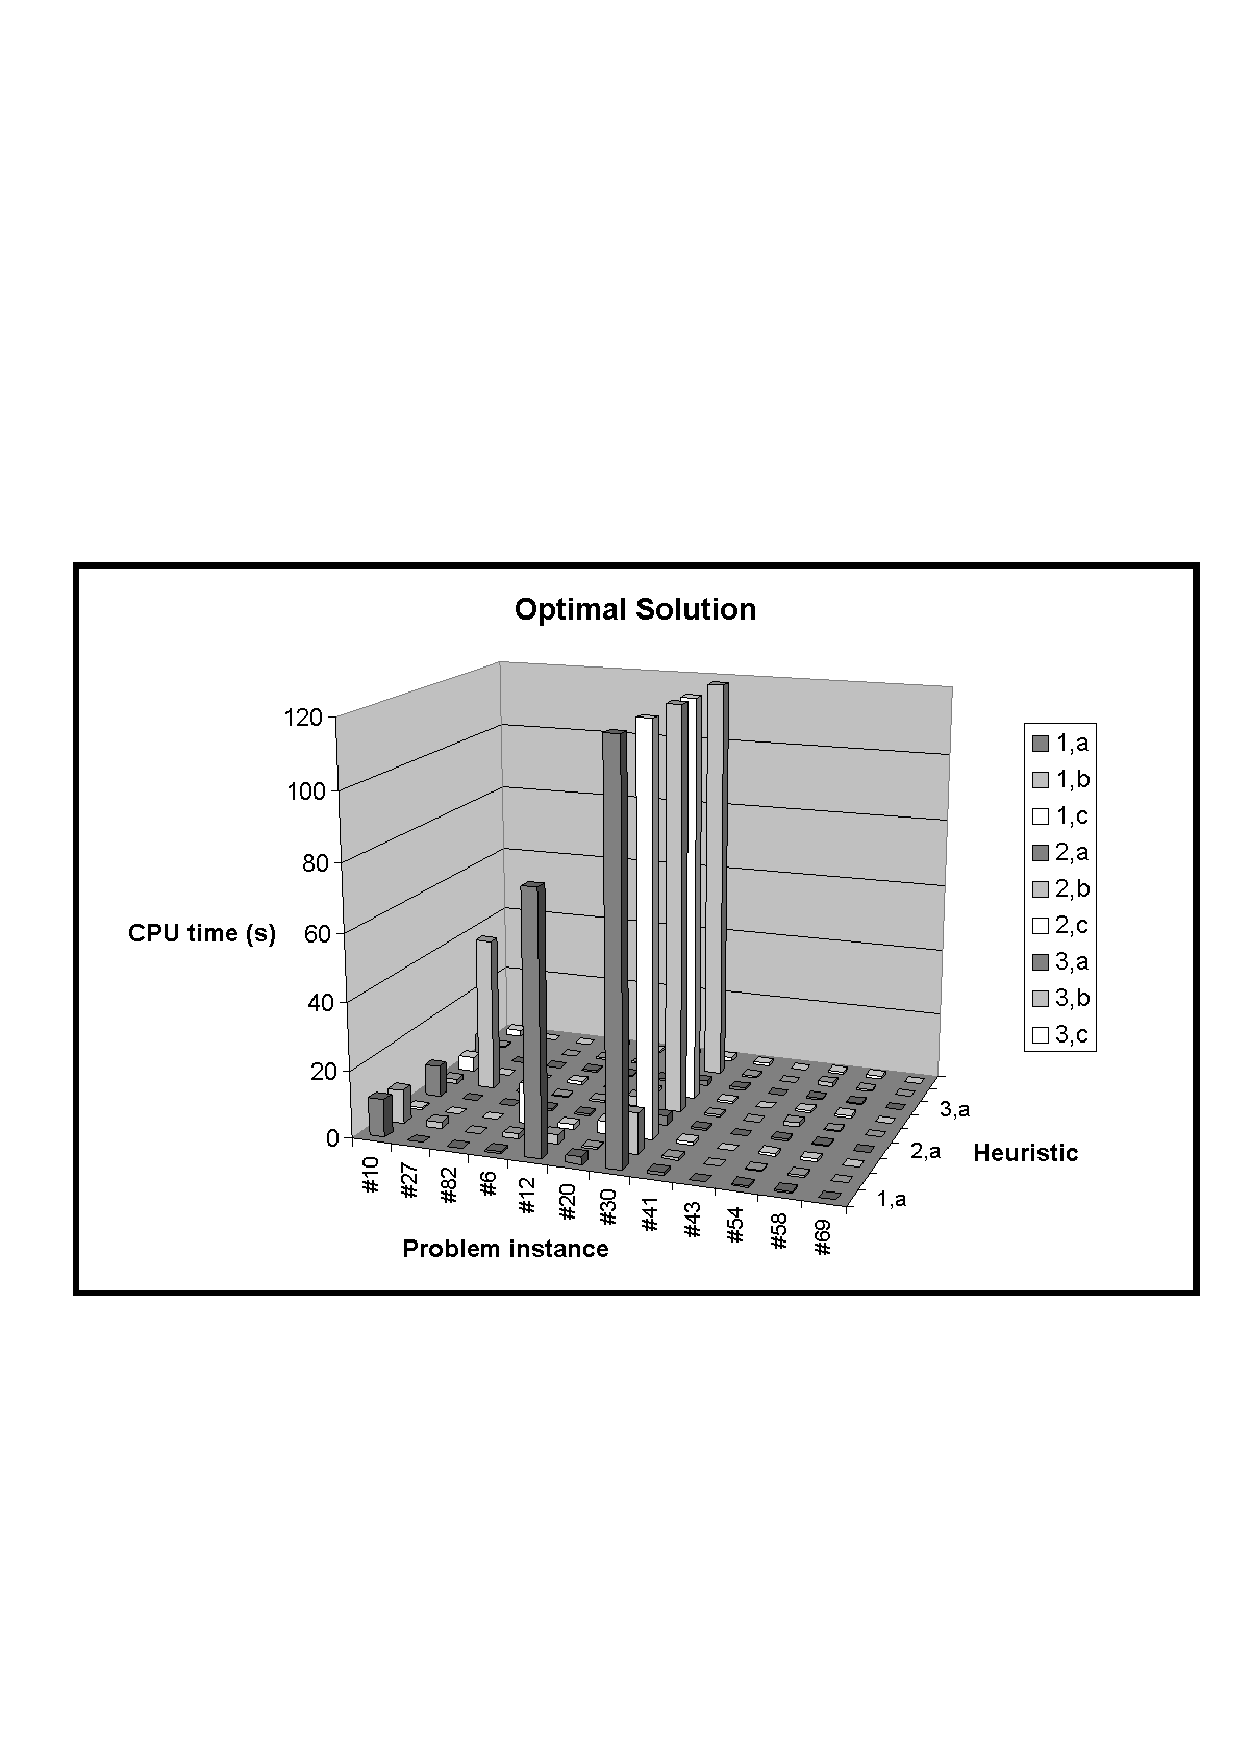
\includegraphics[width=32pc]{figures/fig10.pdf}}
\caption{Effect of heuristic for finding optimal solution}
\label{fig10}
\end{figure}

\begin{figure}
\centerline{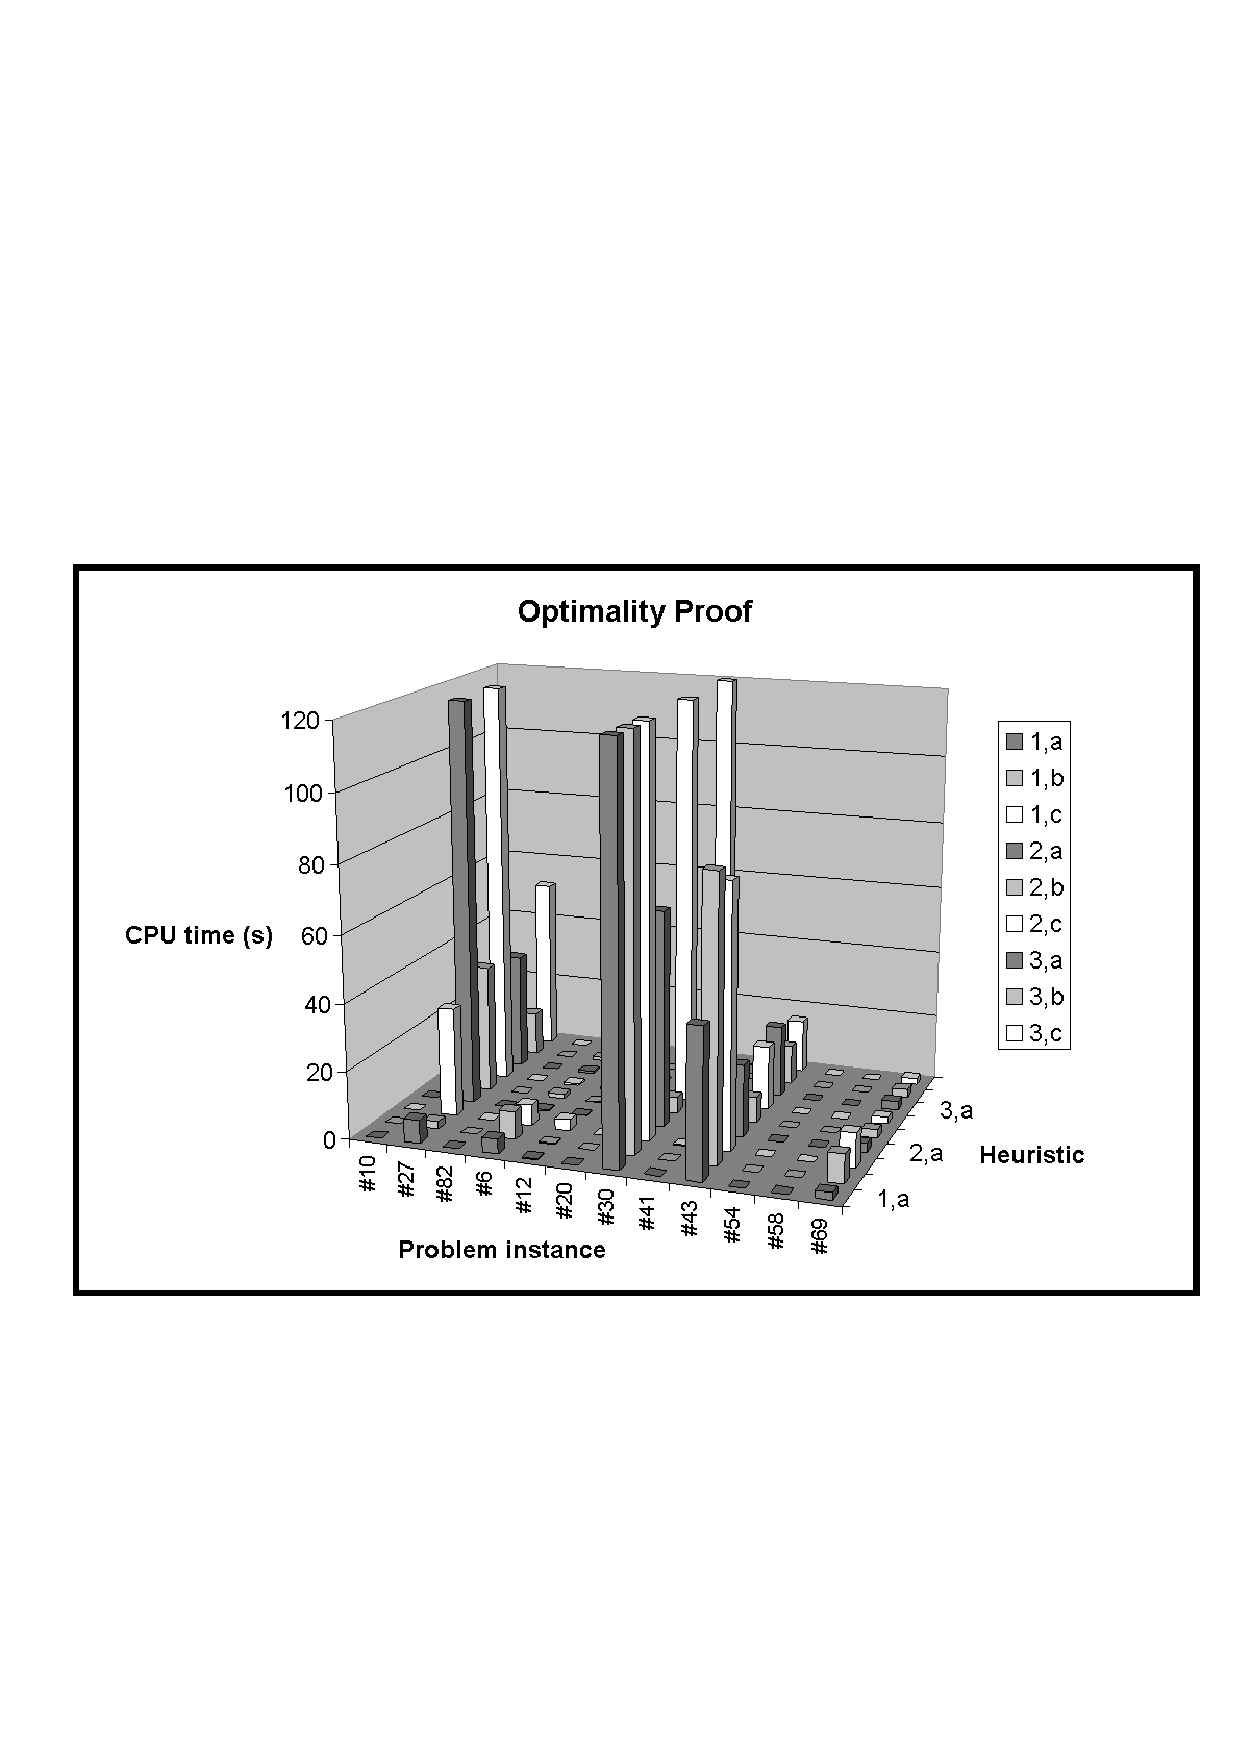
\includegraphics[width=32pc]{figures/fig11.pdf}}
\caption{Effect of heuristic for proving optimality}
\label{fig11}
\end{figure}

If in  these tests we  switch off the  part of the  balance constraint
that is responsible   for discovering  new precedence  relations  (see
section \ref{dnpr}), only 6  out  of the  12 problem instances  can be
solved to  optimality in less  than 2mn CPU  time.  This suggests that
the discovery of  new precedence  relations  between events plays   an
important  role in the propagation of  the balance constraint. This is
not very surprising as these new precedence relations result in a more
accurate precedence graph that  will help the  following cycles of the
balance constraint.

\begin{figure}
\centerline{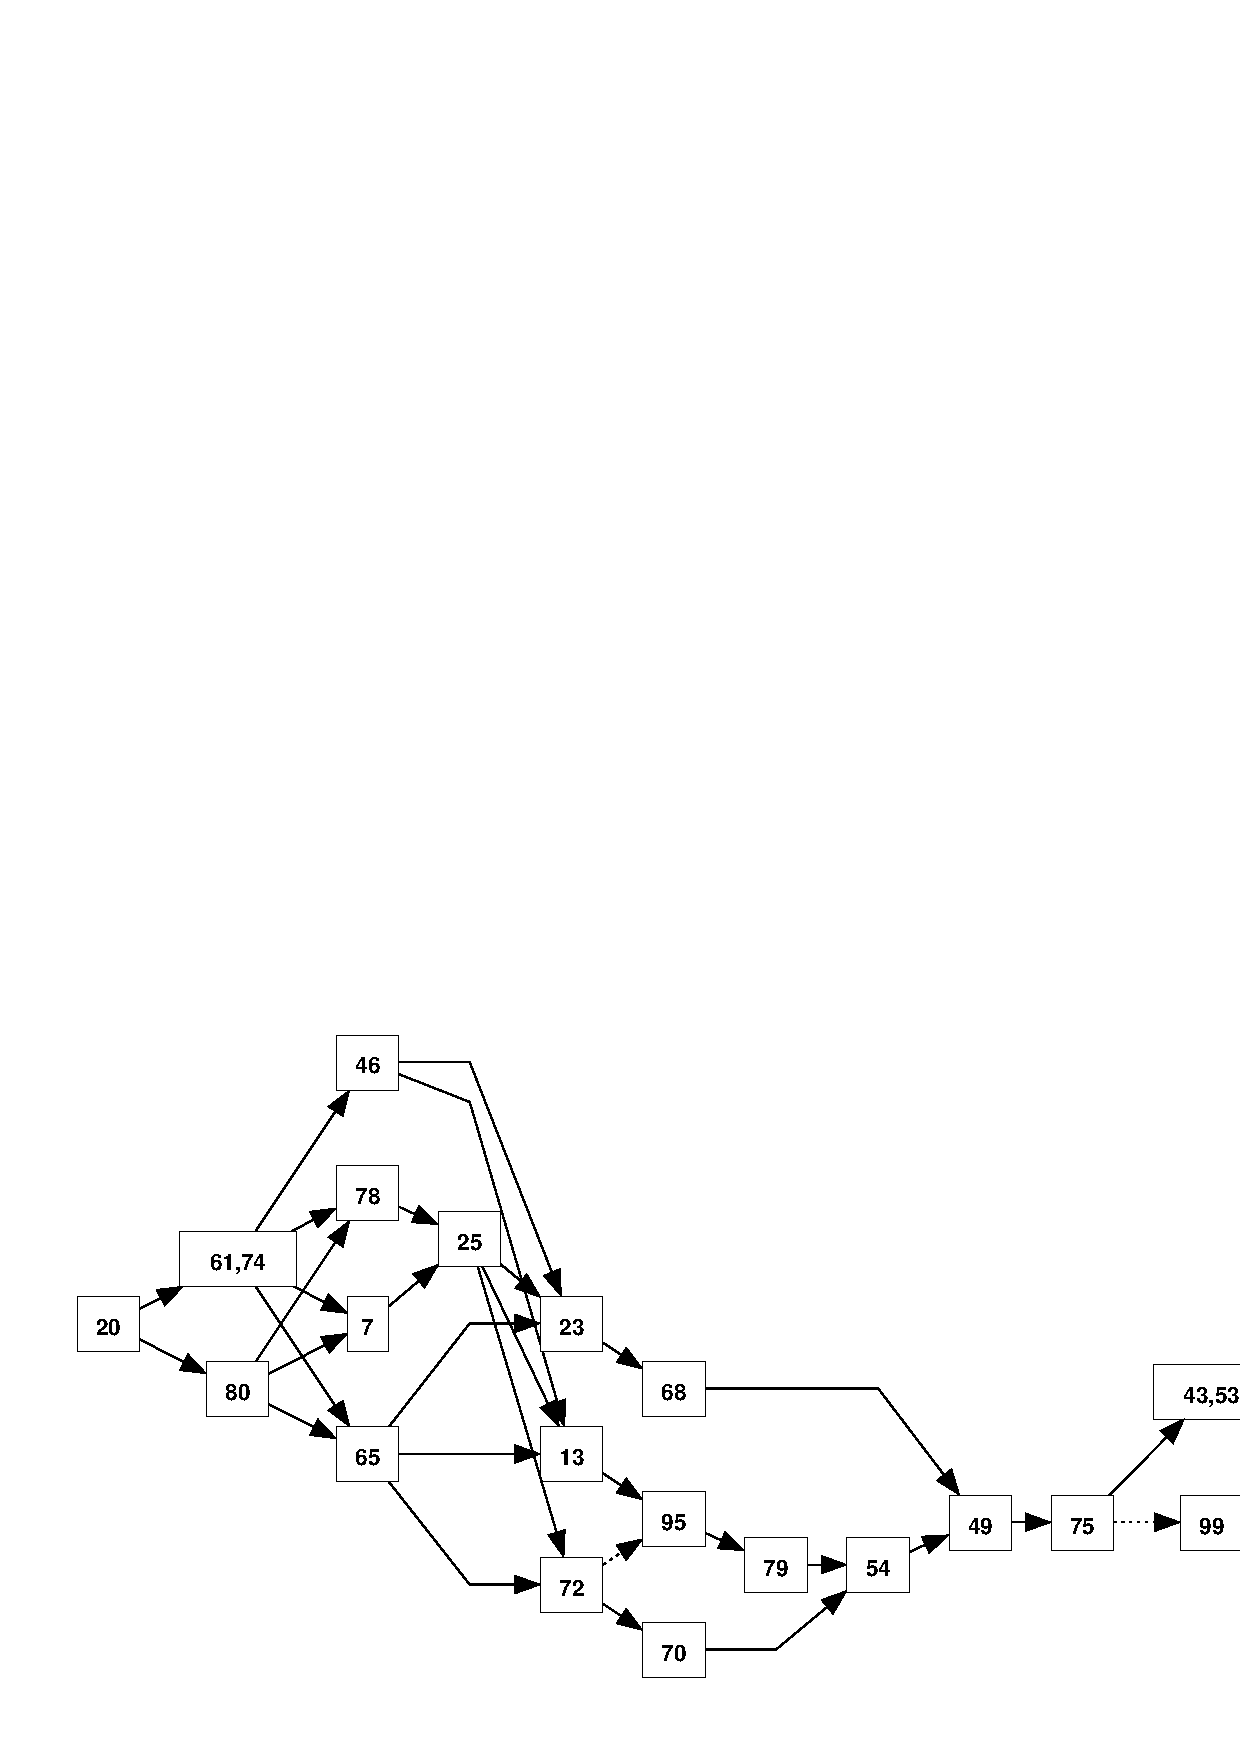
\includegraphics[width=35pc]{figures/fig12.pdf}}
\vspace*{-8mm}
\caption{Part of an optimal solution to instance \#41}
\label{fig12}
\end{figure}

\subsection{Energy Precedence Constraint}

The main  strength  of the energy  precedence  constraint is  to allow
propagation even when  the time window   of activities is very  large.
This is, for instance, typically the case  in pure scheduling problems
with makespan minimization when searching for a good first solution in
the absence of tight upper bound on makespan.   In our experiments, we
focused on jobshop  problems (unary resources)  because a considerable
effort has  been devoted in the past  forty years to  design heuristic
greedy  procedures for solving job-shop problems  so there is a lot of
material to  compare with.  For this purpose,  we  wrote a very simple
least-commitment search procedure based  on the precedence  graph that
orders pairs of  activities  on a unary resource  and  aims at finding
very  good  first  solutions\footnote{The   C++ code  of   this search
procedure  is  available in the  distribution of  {\em  ILOG Scheduler
5.2}.}.

On  a given  unary resource,  the level  of commitment of  ordering an
activity   $A$ before  and activity  $B$   is estimated as:  $commit(A
\preceq B) =  commit (end(A) \leq  start(B))$ as  described in section
\ref{tempcommit}.  The search   procedures   looks for  the  pair   of
activities $\{A,B\}$ still unranked on a unary resource that maximizes
the   criterion: \[crit(\{A,B\})   = \min(u(A),u(B))  \cdot  |commit(A
\preceq   B)-commit(B \preceq A)|  \]  where  $u(X)$ is  the number of
activities still unranked with respect   to activity $X$ on the  unary
resource. For such a pair  of activities, we can  hope that one of the
ordering induces much less commitment than the  opposite one and that,
as the activities $A$ and $B$ are in a part of the schedule where many
activities are still unranked, posting  the least commitment  ordering
will have  less impact on the schedule.   The search  procedure can be
seen  as a  greedy  algorithm:  it   iteratively selects  the  pair of
activities $\{A,B\}$ that maximizes $crit(\{A,B\})$ and post the least
commitment ordering.  As   at each step,  we select  a local potential
conflict (pair of activities) that can be solved with a minimal impact
on the  other activities,  this search  procedure is expected  to find
solutions where  the domain   of  the  start  and  end   variables  of
activities is  still   very  large.  If    there is  an   optimization
criterion, these large domains leave room for optimizing it.

We tested   this greedy search  procedure with  the  energy precedence
constraint alone (LCEP) on   45 job-shop problems  for which  we could
compare  with other algorithms  (namely:  abz5-6, ft6,  ft10, ft20 and
la1-40). For our tests, we used a schedule horizon equal to the sum of
the duration of  all the activities, which  is of course a  very large
upper  bound  on  the optimal  makespan.  The   average deviation from
optimal makespan (or from best known lower  bound on optimal makespan)
of the  solution produced by our greedy  algorithm is only 5.3\%. This
result is to be compared with  some state-of-the art and/or well-known
greedy algorithms for  solving jobshop problems\footnote{We focus here
on  a comparison with similar procedures  that do not explore a search
tree, that  are not  randomized  and that  are  executed in   a single
pass.}.  In \cite{dellamico93},  a  bidirectional greedy  algorithm is
proposed  (BIDIR)     that  builds  the    schedule   from  both sides
(chronologically  and  anti-chronologically).  In \cite{caseau95}, the
authors describe  a chronological scheduling  procedure (GREEDY) based
on a  look-ahead technique that select the  next operation to schedule
as the one  that is  expected to  increase as  little as possible  the
makespan. We also compared our approach with a  single pass of the PCP
algorithm  proposed in  \cite{cheng97} using  the  same loose  initial
upper bound as for  LCEP (sum of the duration  of all the activities).
In this paper, the authors start from an  initial upper bound given by
the  application of six  priority rules (SPT,LPT,LFT,EFT,MOR,LOR).  We
also compare our approach with this upper bound (6RULES). As far as we
know,      the   best   greedy   algorithm        so far   is     AMCC
\cite{pacciarelli99}. AMCC selects the pair of activities $(A,B)$ such
that posting $A  \preceq  B$ would  increase as  much as  possible the
current lower bound on makespan and then  post the opposite constraint
$B \preceq  A$.  The average  deviation from  optimal makespan of  all
these  procedures is given on  Figure \ref{fig18}.  Note that when the
energy precedence   constraint    is not used  (LCNEP),    the average
deviation of our  greedy search procedure increases  up to 10.9\%.  It
shows  that  the    energy  precedence  constraint  allows    a strong
propagation when the domain of activities  is not very tight.  Because
of this   additional propagation, the   heuristics for  estimating the
level of commitment are more informed and lead  to better results.  As
expected,  we noticed that the usage  of  the timetabling, disjunctive
and/or edge-finding   constraint has  strictly  no   influence on  the
quality of the solution found by our search  procedure given the large
horizon of the schedule.

\begin{figure}
\centerline{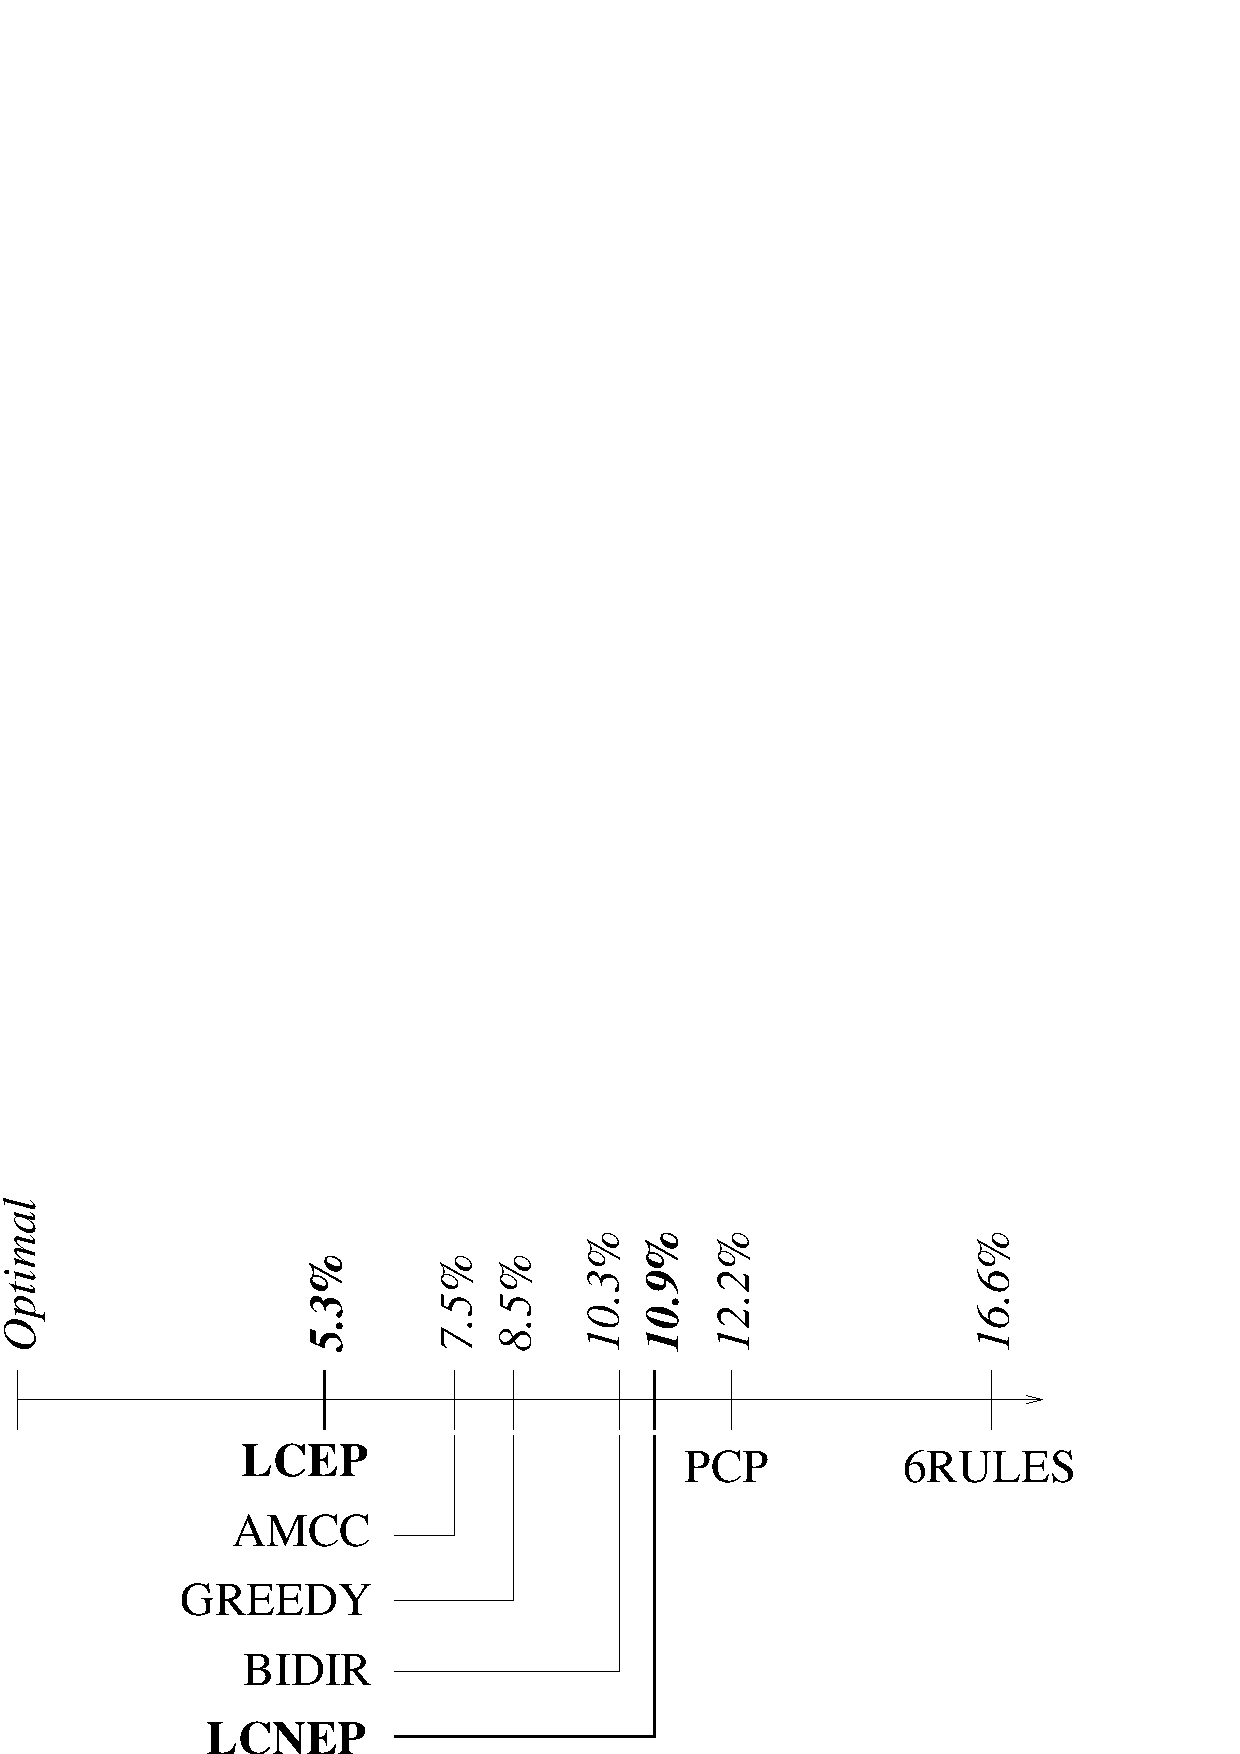
\includegraphics[width=20pc]{figures/fig18.pdf}}
\caption{Average deviation from optimal of some greedy single-pass algorithms}
\label{fig18}
\end{figure}


\section{Balance Constraint Extensions \label{extensions}}

\subsection{Balance Constraint as a First Order Approximation of
Resource Level \label{orderk}}

We  show  in this  section  how  the levels   computed by the  balance
constraint    $L^{<}_{max}(x)$,  $L^{>}_{max}(x)$,   $L^{<}_{min}(x)$,
$L^{>}_{min}(x)$  can be seen  as a  first order  approximation of the
actual level of the reservoir just before and after event $x$.

For symmetry  reasons, we focus  only on $L^{<}_{max}(x)$.  As seen in
formula (\ref{formula2})  in  section \ref{newbounds},   this level is
defined as follows:

\begin{displaymath}
L^{<}_{max}(x) = \lambda(x) + \mu_1(x) ~\textrm{where}~
\left\{ \begin{array}{l}
\displaystyle \lambda(x) = \sum_{y \in B(x)} q_{max}(y)\\
\displaystyle \mu_1(x) =  \sum_{y \in P \cap (BS(x) \cup U(x))} \hspace{-10mm} q_{max}(y)
\end{array} \right.
\end{displaymath}

$\lambda(x)$ represents    the maximal contribution  to  the reservoir
level  of those events that  are certainly  before event $x$. Provided
the reservoir variables $q$ are independent, this maximal contribution
is evaluated exactly by $\lambda(x)$.

$\mu_1(x)$ represents the contribution to the reservoir level of those
events  that are  still not ranked    with respect to  event  $x$. The
formula  to   compute  $\mu_1(x)$ is  an upper   bound  of  the actual
contribution.  It can be  seen as the exact  contribution of a relaxed
problem where  all  the  precedence  relations between  events  in the
subset  $BS(x)  \cup U(x)$ are  ignored. In  that  case, indeed, it is
possible to execute all the producing events  $y$ of $BS(x) \cup U(x)$
strictly before $x$ and all the consuming  events of $BS(x) \cup U(x)$
simultaneously or after $x$.

But we could  compute a much better  estimation of the contribution of
those events that are still not ranked  with respect to event $x$. The
idea is to  apply the balance  constraint to  the subgraph $\Psi(x)  =
BS(x) \cup U(x)$. 

Let's illustrate this idea by an example. Suppose the precedence graph
of  Figure \ref{fig6}. We  are interested in  computing an estimate of
the level  of reservoir just  before event $x$. The balance constraint
would compute a level  $L^{<}_{max}(x)=4$ as $\lambda(x)=(+2-1)=1$ and
$\mu_1(x)=(+1+2)=3$.  A second-order   estimate of the   maximal level
just before  $x$ consists in  applying  the balance constraint  on the
subgraph $\Psi(x)=BS(x)\cup  U(x)$ shown  in the  figure.   The levels
resulting  from  the  application  of the  balance  constraint on this
subgraph are  represented in italic.   For  any instantiation of  time
variables  compatible with the  precedence  graph, either (1) all  the
events in $\Psi(x)$  are scheduled  strictly  before $x$ or (2)  there
exists some event $y_0 \in \Psi(x)$ (not necessarily unique) such that
$y_0$ is the first event of $\Psi(x)$ to be executed simultaneously or
after  $x$ in the instantiation.   In the first case, the contribution
of  the events of $\Psi(x)$  to the level  just before  $x$ is exactly
equal to $\sigma_x  = \sum_{y\in  \Psi(x)}q_{max}(y)$.  In the  second
case,  the level  $L^{<}_{max}(y_0,\Psi(x))$  computed  by the balance
constraint before $y_0$ on $\Psi(x)$ is clearly  an upper bound of the
contribution  of $\Psi(x)$.  As   a  conclusion, the maximal value  in
$\{\sigma_x,\{L^{<}_{max}(y,\Psi(x))\}_{y\in  \Psi(x)} \}$  is a valid
upper  bound for the contribution of  $\Psi(x)$ to the reservoir level
at  date $t(x)-\epsilon$.  In the example,  we have $\sigma_x = 0$ and
the  values for $L^{<}_{max}(y,\Psi(x))$  are $\{ 0, 1,  1,  -1, 1 \}$
thus, an upper bound on the contribution  of $\Psi(x)$ is evaluated as
$\mu_2(x) = 1$ which  gives an  upper  bound of $2$ for  the reservoir
level just before event $x$. This upper bound of $2$ can be contrasted
with the   upper bound  $4$  computed  by  the $1^{st}$-order  balance
constraint.

\begin{figure}
\centerline{\includegraphics[width=22pc]{figures/fig6.pdf}}
\caption{Example of second order approximation of resource levels}
\label{fig6}
\end{figure}

To express more formally the recurrence relation implied by this idea,
we need to extend our notation slightly. Let  $\Omega$ be a subset of
events on the reservoir and  $\Psi(x,\Omega) = \Omega \cap (BS(x) \cup
U(x))$.  The level computed by the   balance constraint on  the set of
events $\Omega$ is given by:

\begin{displaymath}
L^{<}_{max,1}(x,\Omega) = \lambda(x,\Omega) + \mu_1(x,\Omega)
\end{displaymath}
\begin{displaymath}
~\textrm{where}~
\left\{ \begin{array}{l}
\displaystyle \lambda(x,\Omega) = \sum_{y \in \Omega \cap B(x)} \hspace{-2mm} q_{max}(y)\\
\displaystyle \mu_1(x,\Omega) =  \sum_{y \in P \cap \Psi(x,\Omega)} \hspace{-5mm} q_{max}(y)
\end{array} \right.
\end{displaymath}

As suggested above, a better estimation of  this level can be computed
as follows:

\begin{displaymath}
L^{<}_{max,i}(x,\Omega) = \lambda(x,\Omega) + \mu_i(x,\Omega)
\end{displaymath}
\begin{displaymath}
~\textrm{where}~
\mu_i(x,\Omega) = \max \left(
\begin{array}{l}
\displaystyle \max_{y \in \Psi(x,\Omega)}{L^{<}_{max,i-1}(y,\Psi(x,\Omega))}\\
\displaystyle \sum_{y \in \Psi(x,\Omega)}{\hspace{-1mm}q_{max}(y)}
\end{array} \right) \hspace{20mm}(3)
\end{displaymath}

Let  $\Omega_0$ denote  the set  of all events  on  the reservoir. The
following results are shown in the appendix:

\proposition{1}{$\forall i$, $L^{<}_{max,i}(x,\Omega_0)$   provides an
upper bound on the reservoir level at $t(x)-\epsilon$.}

Let $p$ denote the maximal degree of parallelism of the precedence
graph; that is, the size of the biggest set  $Q \subset \Omega_0$ such
that $\forall x,y \in Q, y \in BS(x) \cup U(x)$.

\proposition{2}{The sequence $L^{<}_{max,i}(x,\Omega_0)$ is decreasing
with index  $i$. Furthermore, after  the index   $p$, the sequence  is
stationary        and  equal   to    a      value    we  will   denote
$L^{<}_{max,\infty}(x,\Omega_0)$.}


\proposition{3}{If the  only constraints are the  precedence relations
in the precedence graph  and the reservoir  maximal level, then, there
exists an instantiation of the variables such that the reservoir level
at        date       $t(x)-\epsilon$    is         equal            to
$L^{<}_{max,\infty}(x,\Omega_0)$.        Stated             otherwise,
$L^{<}_{max,\infty}(x,\Omega_0)$  is   the best  upper   bound on  the
reservoir level just before event $x$.}

Let's assume  $|\Psi(x,\Omega)| = \beta  \cdot |\Omega|$  where $\beta
\in [0,1)$.

\proposition{4}{$L^{<}_{max,i}(x,\Omega_0)$  can  be  computed  with  a
polynomial        algorithm      whose    complexity      is        in
$O(\beta^{\frac{i(i+1)}{2}-1}\, n^i)$.}

\proposition{5}{$L^{<}_{max,\infty}(x,\Omega_0)$ can be  computed with
an     algorithm   whose    complexity     is    in   $O(n^{-\frac{\ln
n}{\ln{\beta}}})$.}

All these results are illustrated in Figure \ref{fig7}.

\begin{figure}
\centerline{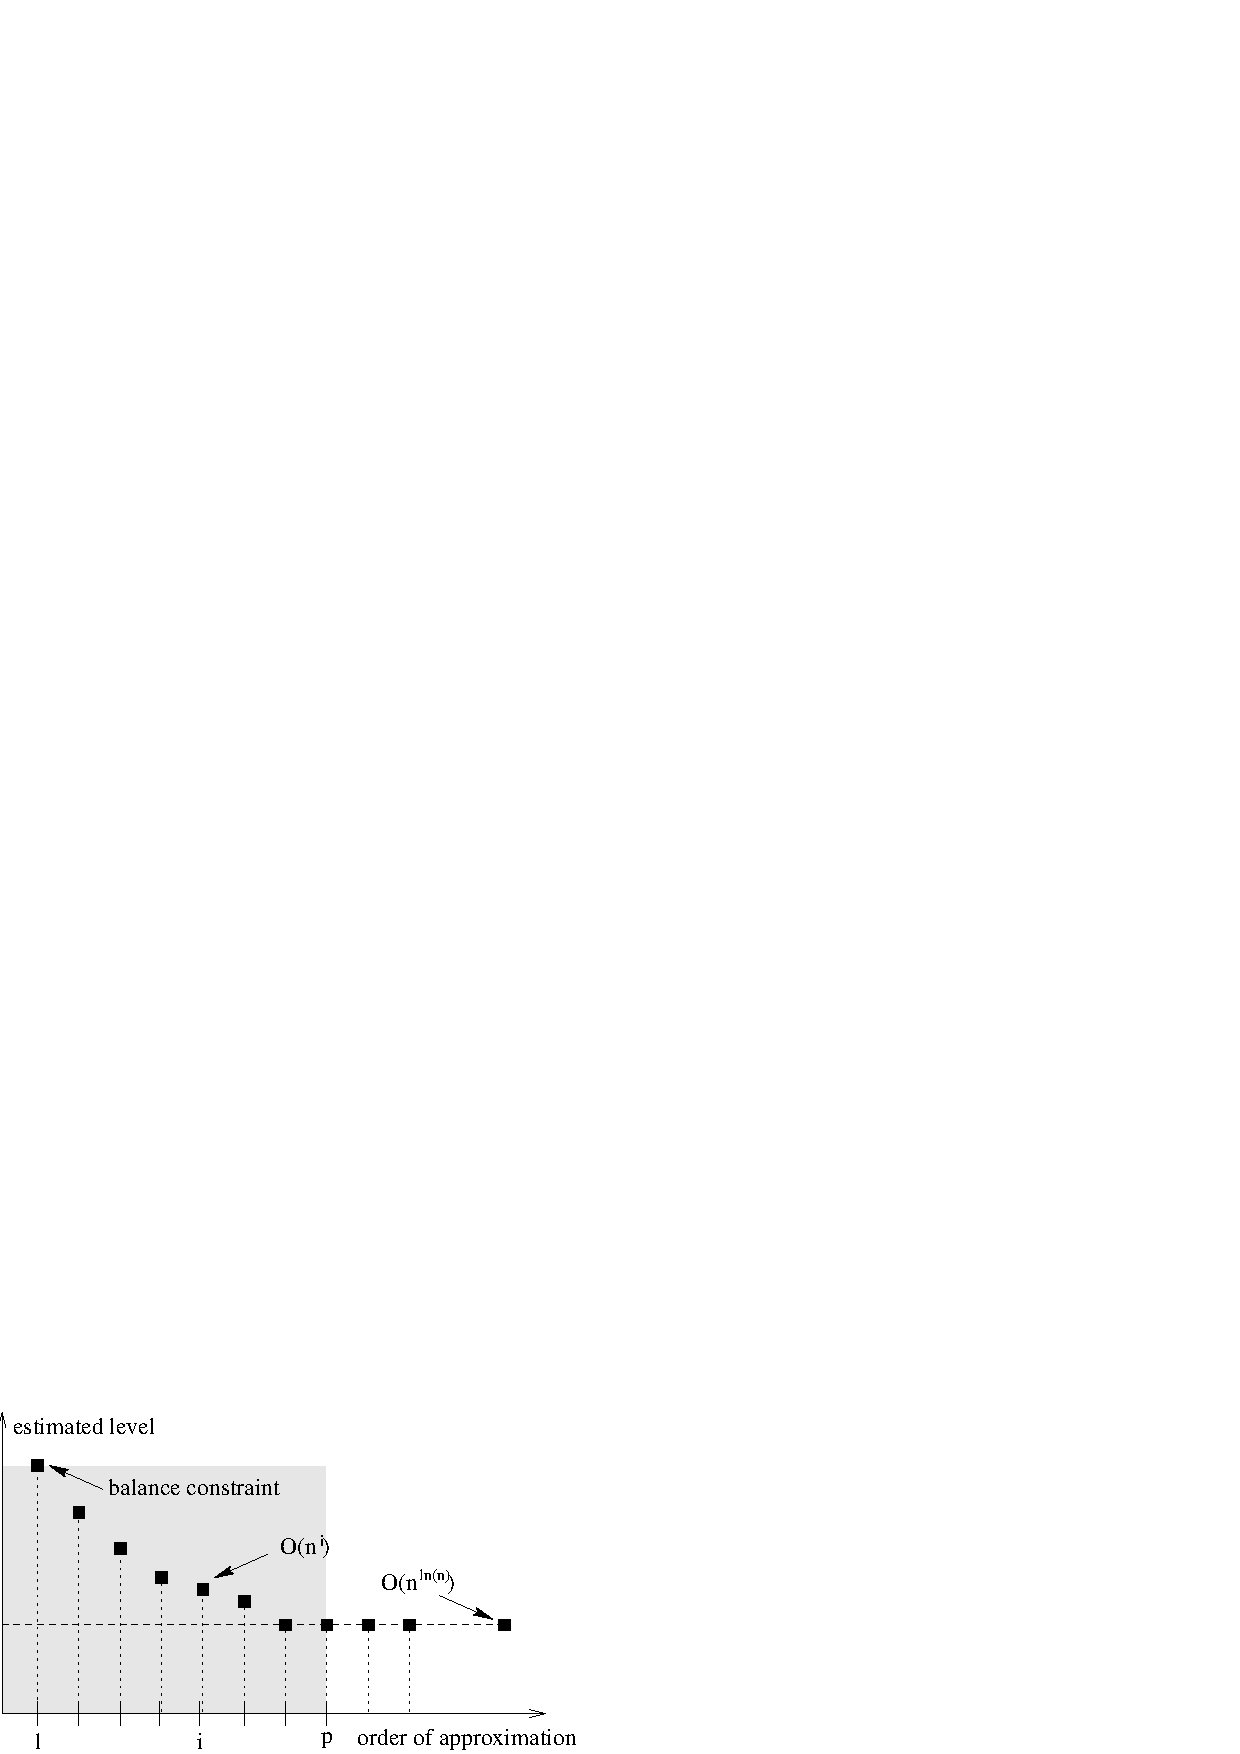
\includegraphics[width=18pc]{figures/fig7.pdf}}
\caption{Computing $i^{th}$-order approximation of resource levels}
\label{fig7}
\end{figure}

The advantages of computing better bounds for the reservoir levels are
clearly to quickly detect dead ends and safe  events (which results in
having  less   unnecessary     precedence    relations    in       the
solutions). Furthermore, it is easy  to see  that all the  propagation
performed   by the balance constraint   (new  bounds on resource usage
variables, new bounds on time variables, new precedence relations) can
be   extended   and   improved  by using    the   levels  computed  on
$\Psi(x,\Omega)$.

The  short   algorithmic complexity  analysis    above suggests  that,
although systematically computing higher approximation orders may turn
out  to  be expensive, it could  be  interesting  to detect situations
where,            for          example,          the               gap
$L^{<}_{max,1}(x,\Omega_0)-L^{<}_{max,2}(x,\Omega_0)$ is large so that
it would be worth using  a  $2^{nd}$-order approximation  for some event
$x$.

Furthermore, in  practice, for  computing $L^{<}_{max,i}(x,\Omega_0)$,
the full recursion suggested by  formula {\it 3}  does not need to  be
completely explored. For example suppose  that for some event $x$, the
list   $(y_1,y_2,...,y_k,...)$  represents   the   set  of  events  in
$\Psi(x,\Omega_0)$            ordered            by         decreasing
$L^{<}_{max,1}(y,\Psi(x,\Omega_0))$. If there   is an index  $i$  such
that             $L^{<}_{max,i}(y_1,\Psi(x,\Omega_0))             \geq
L^{<}_{max,1}(y_2,\Psi(x,\Omega_0))$           then         \linebreak
$L^{<}_{max,i}(x,\Omega_0)=\lambda(x,\Omega_0)                       +
L^{<}_{max,i}(y_1,\Psi(x,\Omega_0))$  as for  all $k  \geq 2$ we  will
have                $L^{<}_{max,i}(y_1,\Psi(x,\Omega_0))          \geq
L^{<}_{max,1}(y_2,\Psi(x,\Omega_0))$                             $\geq
L^{<}_{max,1}(y_k,\Psi(x,\Omega_0))$         \linebreak          $\geq
L^{<}_{max,i}(y_k,\Psi(x,\Omega_0))$. In  other  words,  in this case,
$L^{<}_{max,i}(y,\Psi(x,\Omega_0))$ does not need  to be computed  for
all the events $y$ in $\Psi(x,\Omega_0)$.

Another  way to improve the  computation is based  on the fact that in
the recurrence    relation, the  value    $L^{<}_{max,i}(x,\Omega)$ is
computed several times for the same  subset $\Omega$. This suggests that
dynamic programming approaches could help reducing the complexity.

Note  also that,  as suggested by  the  comparison with MCSs evoked in
section            \ref{balance},       the     computation         of
$L^{<}_{min,\infty}(x,\Omega_0)$          (and           symmetrically
$L^{<}_{max,\infty}(x,\Omega_0)$) can be  reformulated  as the  search
for a critical set  that maximizes resource consumption.  This problem
can be seen as the search for a maximum  weighted independent set on a
comparability graph\footnote{The   graph whose       edges   represent
precedence relations between activities requiring  the resource.}.  As
shown   in  \cite{ford62},   there  exists   efficient polynomial-time
algorithms  that run  in  $O(n^{1.5}\sqrt{m/\log(n)})$  to solve  this
problem.  The adaptation of  these algorithms to compute better bounds
on the reservoir levels is part of our future works.

\subsection{Toward a real plan generation procedure \label{truthcriterion}}

This section outlines  a planning search procedure  that relies on the
levels computed   by the  balance   constraint (at  $1^{st}$-order  or
higher) to generate a plan. 

It should   be noted  than   in a  typical planning problem,  resource
attributes have to be handled  together with pre-condition achievement
on  classical attributes.  As   proposed  in \cite{laborie95}, we  can
distinguish between  several  types   of  flaws on the   partial  plan
(unexplained  propositions,  threads   and resource   conflicts).  The
opportunity to solve a  given flaw can  be estimated independently  of
the nature of   this   flaw (unexplained  propositions,   threads  and
resource conflicts).   The  global search algorithm  then  consists in
selecting  the most opportunistic flaw   to be solved  at the  current
search node and  branching on its  possible  resolvers.  This approach
leads to a natural integration of the processes of plan generation and
scheduling as some opportunistic scheduling decisions are taken before
the whole plan is generated.

In this section, we focus on the definition of flaws on reservoirs and
their resolvers. Let $s$ be the current state on  a given reservoir of
maximal level $Q$.   For a given event  $x$, the possible positions of
the levels $L^<_{min}(x)$ and $L^<_{max}(x)$ with respect to the level
interval  $[0,Q]$ is depicted  in  Figure \ref{fig13}.  Note that  for
symmetry   reasons, we do not   consider the levels $L^>_{min}(x)$ and
$L^>_{max}(x)$.

\begin{figure}
\centerline{\includegraphics[width=20pc]{figures/fig13.pdf}}
\caption{Potential flaws on reservoir}
\label{fig13}
\end{figure}

Except for case (\texttt{A})  where the event  is  safe, each  case in
Figure \ref{fig13} corresponds to a potential flaw of the current plan
where the reservoir could  underflow or/and overflow.  The basic tools
to solve  potential  flaws are  either: (V)  to  reduce  the domain of
reservoir usage  variables $q$,  (T)  to add new  precedence relations
between events or (O) to insert in the plan new operators that contain
some events on  the reservoir. The idea consists  in using those basic
tools to bring the bounds $L^<_{min}(x)$  and $L^<_{max}(x)$ back to a
situation  where  event  $x$  is safe,    that is,  as  shown  in case
(\texttt{A}): $0 \leq L^<_{min}(x)$ and $L^<_{max}(x)\leq Q$.

For symmetry reason, we only consider cases (\texttt{B}), (\texttt{C})
and (\texttt{D}).

{\bf Case (\texttt{B}).}   In this case, it  is clear that at least  a
consuming   event  $y$ must  be  inserted  strictly  before event $x$.
Indeed, if no  planning operator is applied  to insert a new consuming
event strictly before $x$,  then,  by definition of $L^<_{min}(x)$  we
are sure that the reservoir will overflow just before $x$. Indeed, the
consuming events unranked  with respect to  $x$ are not sufficient  to
prevent  the reservoir  overflow.   The  analogous  case in  classical
partial order planning is when no action  currently exists in the plan
to ensure  a given pre-condition; in this  case, a  new action must be
inserted. This can be stated as follow:

\[\exists y \in new\_op \ / \ new\_op \notin s, y \in new\_op, q(y)<0,
t(y)<t(x) \qquad | \  \textrm{(O)}\]

{\bf Case (\texttt{C}).} In this case,  as $L^<_{min}(x)\leq Q$, it is
possible that a monotonic change (Q) or (T) will result in a situation
where  $L^<_{max}(x)\leq    Q$.  It will   consist   in decreasing the
reservoir production before $x$ or  stating that an existing consuming
event must  be  executed strictly   before  $x$ or that  an   existing
producing  event cannot be  executed strictly  before $x$.  Of course,
inserting  a  consuming  event  strictly  before   event $x$ is   also
possible.

\begin{displaymath}
\lor
\left\{ \begin{array}{l}

\left. \begin{array}{l}
\exists y \in B_s(x) \ / \ q(y) < q_{max,s}(y) \qquad \\
\exists y \in P \cap \Psi_s(x) \ / \ q(y) < q_{max,s}(y) \qquad \\
\end{array} \right|
\  \textrm{(V)}\\

\left. \begin{array}{l}
\exists y \in C \cap \Psi_s(x) \ / \ t(y) < t(x) \qquad \\
\exists y \in P \cap \Psi_s(x) \ / \ t(y) \geq t(x) \qquad \\
\end{array} \right|
\  \textrm{(T)}\\

\exists y \in new\_op \ / \ new\_op \notin s, y \in new\_op, q(y)<0,
t(y)<t(x) \qquad | \  \textrm{(O)}\\

\end{array} \right.
\end{displaymath}

{\bf Case (\texttt{D}).} This case is the union of case (C) with
its symmetrical case on the reservoir underflow. That is:


\begin{displaymath}
\lor
\left\{ \begin{array}{l}

\left. \begin{array}{l}
\exists y \in B_s(x) \ / \ [q(y) < q_{max,s}(y)] \lor [q(y) > q_{min,s}(y)]\qquad \\
\exists y \in P \cap \Psi_s(x) \ / \ q(y) < q_{max,s}(y) \qquad \\
\exists y \in C \cap \Psi_s(x) \ / \ q(y) > q_{min,s}(y) \qquad \\
\end{array} \right|
\  \textrm{(V)}\\

\exists y \in \Psi_s(x) \ / \ [t(y) < t(x)] \lor [t(y) \geq t(x)]
\qquad | \  \textrm{(T)}\\

\exists y \in new\_op \ / \ new\_op \notin s, y \in new\_op, t(y)<t(x)
\qquad | \  \textrm{(O)}
	
\end{array} \right.
\end{displaymath}

The complexity  of computing this criterion for  a given  event $x$ is
clearly    in $O(n)$  in worst  case    if the levels  $L^<_{min}(x)$,
$L^<_{max}(x)$,  $L^>_{min}(x)$  and   $L^>_{max}(x)$  are  the   ones
computed by the balance constraint.

Let's   illustrate   the   underlying     search   procedure  by    an
example.   Suppose  a reservoir of   maximal  capacity $Q=10$ with two
initial events $c_0$ and $p_0$ such that $q(c_0)=-5$, $q(p_0)=+10$ and
$t(c_0) < t(p_0)$. The precedence graph  on this reservoir is shown in
Figure \ref{fig14}. Suppose also that there exists two operators $O_p$
and    $O_c$: $O_p$   contains  a   production  event  $p$ such   that
$q(p)\in[+3,+4]$, and $O_c$ contains a consumption  event $c$ such that
$q(c)\in[-2,-1]$.

\begin{figure}
\centerline{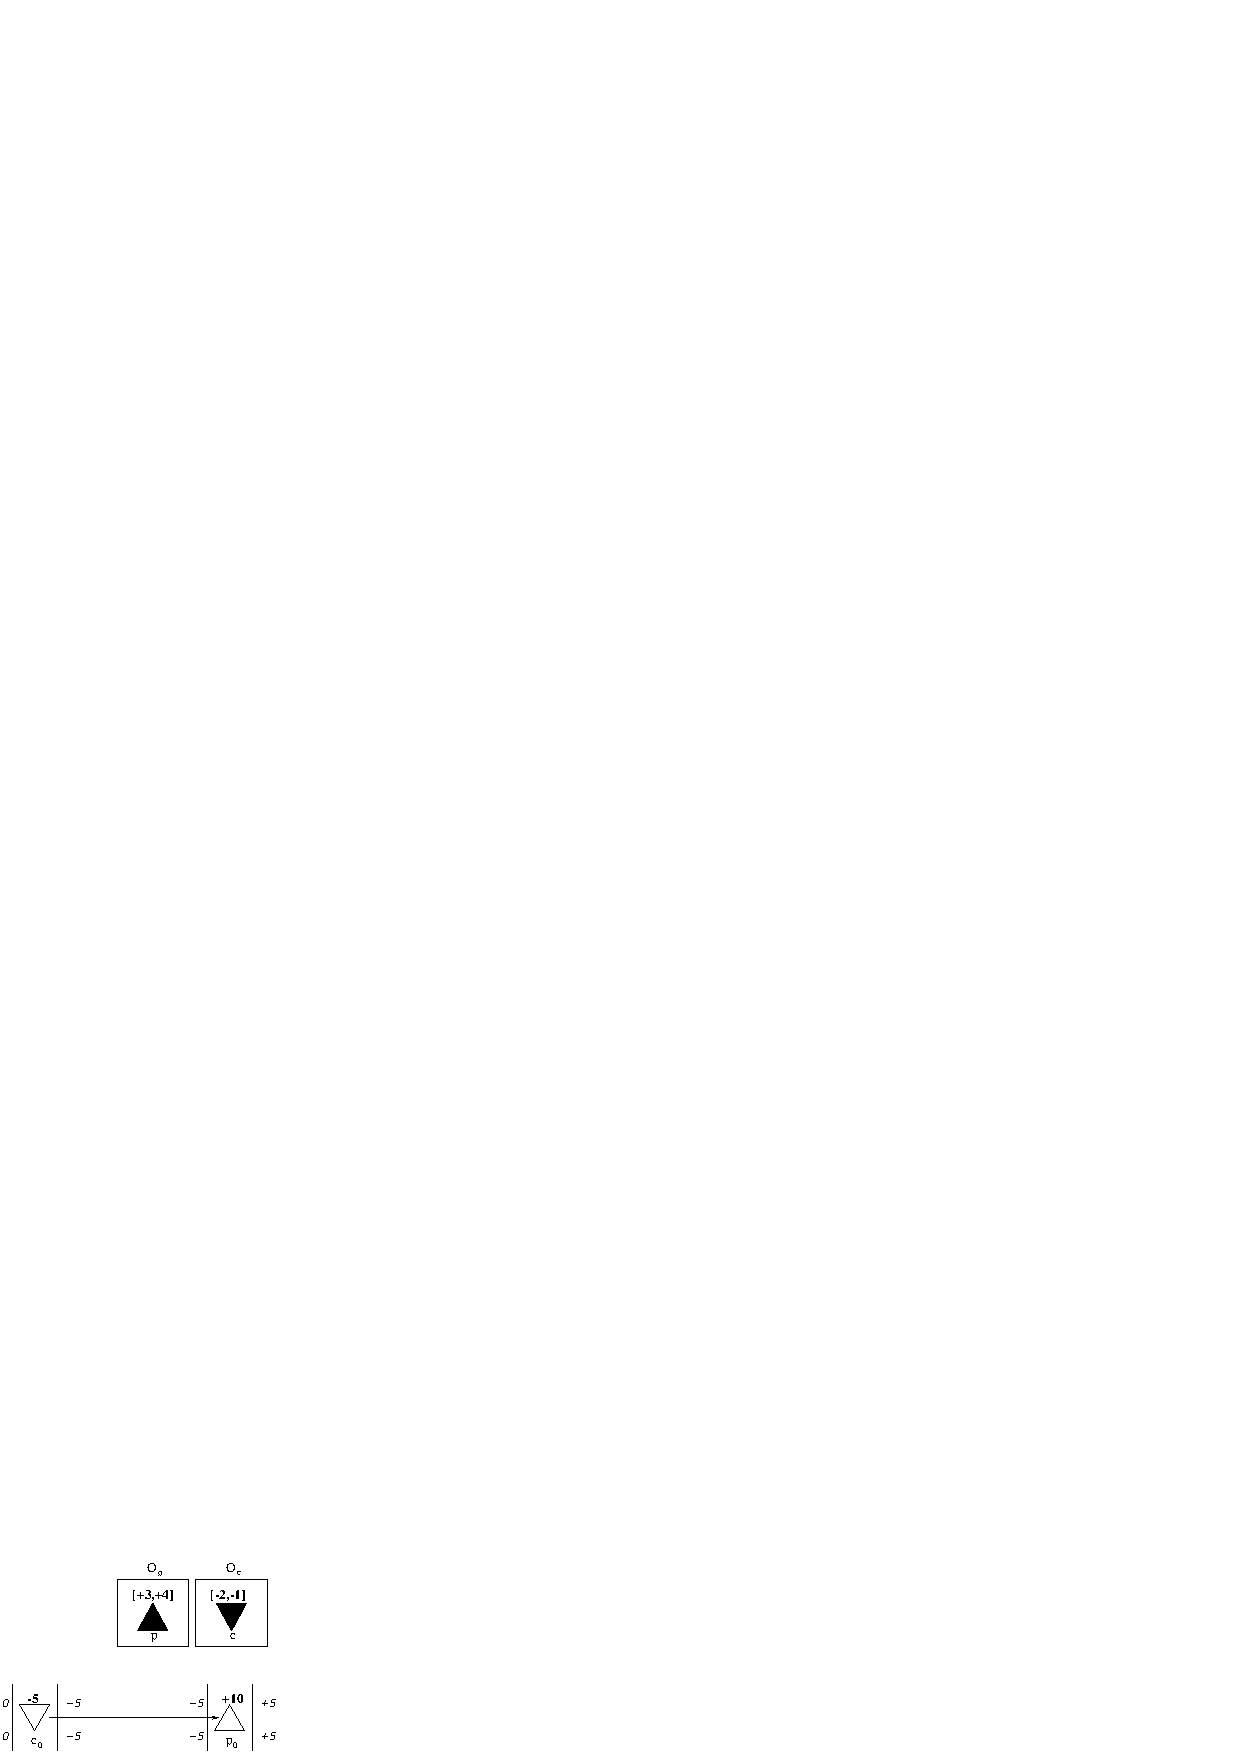
\includegraphics[width=11pc]{figures/fig14.pdf}}
\caption{Initial plan}
\label{fig14}
\end{figure}

The   levels   $L^<_{min}(x)$,    $L^<_{max}(x)$,  $L^>_{min}(x)$  and
$L^>_{max}(x)$  are represented for each event in the figure. One can
notice that the  reservoir level  just before  $c_0$ is  in  situation
(\texttt{A}), and in  situation (\texttt{E}) just after. The reservoir
level just before $p_0$ is in situation (\texttt{E}), and in situation
(\texttt{A}) just after. Thus, there are two potential flaws: one just
after   $c_0$  and   one just before     $p_0$.   Case (\texttt{E}) is
symmetrical  to case (\texttt{B})   and when applied just  after event
$c_0$, it enforces  the insertion of  an instance of operator $O_p$ in
the current plan  before event $c_0$.  In the next  state, we can  see
that the reservoir  level just after $c_0$ is  estimated to  belong to
$[-2,-1]$, thus it   is still in  situation  (\texttt{E})  and another
instance  of operator $O_p$  needs to be   inserted. This leads to the
current plan of Figure \ref{fig15}.

\begin{figure}
\centerline{\includegraphics[width=18pc]{figures/fig15.pdf}}
\caption{Plan after insertion of two instances $p_1$, $p_2$ of $O_p$ before $c_0$}
\label{fig15}
\end{figure}

We  see  now   that event  $p_0$   is  in  situation  (\texttt{B})  at
$t(p_0)+\epsilon$ which   justifies the insertion   of an  instance of
operator $O_c$ before $p_0$. This leads to  the current plan in Figure
\ref{fig16}. Note that, so far, no choice point has been created.

\begin{figure}
\centerline{\includegraphics[width=18pc]{figures/fig16.pdf}}
\caption{Plan after insertion of one instances $c_3$ of $O_c$ before $p_0$}
\label{fig16}
\end{figure}

Now, we can consider, for example,  event $c_0$  which is in  situation
(\texttt{F}) at  $t(c_0)-\epsilon$. Here,  there  are several  ways to
reduce  the  potential  flaw.  In   the  current  situation,  we  have
$B(c_0)=\emptyset$, $\Psi(c_0)=\{p_1,  p_2, c_3\}$, thus the procedure
will branch on the following decisions:

\begin{displaymath}
\lor
\left\{ \begin{array}{l}

q(c_3) > -2  \qquad | \  \textrm{(V)}\\

\left. \begin{array}{l}
t(p_1) < t(c_0)\qquad \\
t(p_2) < t(c_0)\qquad \\
t(c_3) \geq t(c_0)\qquad \\
\end{array} \right|\  \textrm{(T)}\\

insert~O_p, p_4 \in O_p, t(p_4) < t(c_0)\qquad | \  \textrm{(O)}\\

\end{array} \right.
\end{displaymath}

The search continues until  all events  are safe.  An example of  final
state of the procedure is depicted in Figure \ref{fig17}.

\begin{figure}
\centerline{\includegraphics[width=20pc]{figures/fig17.pdf}}
\caption{A final plan}
\label{fig17}
\end{figure}

We  can   show that   the  planning search    procedure based   on the
non-deterministic criterion  described  in this section  is  sound and
complete. More precisely, if we define a  final state of the procedure
as a partial state reachable by the procedure where all the events are
safe then two properties hold:
\begin{itemize}
\item {\em Soundness.} A fully instantiated solution plan can be built
      in polynomial time from any final state of the procedure.
\item {\em Completeness.}   If  a fully   instantiated  solution  plan
      exists, then there exists a final state of the procedure.
\end{itemize} 

Furthermore, all the changes on reservoir usage variables (V) and time
variables   (T) introduced   by the   search  procedure  are  strictly
monotonic: they  reduce the  domain  $[L^<_{min}(x),L^<_{max}(x)]$.  A
corollary of this property is that in the case that no operator can be
inserted in the plan (pure scheduling), the search space is finite and
the search procedure will terminate  as for each $x$,  the size of the
domain $[L^<_{min}(x),L^<_{max}(x)]$ is finite.


\section{Conclusion and Future Work}

This paper describes    two new algorithms  for propagating   resource
constraints on  discrete resources  and reservoirs.  These  algorithms
strongly exploit  the temporal relations in  the  partial schedule and
are able to propagate even if the time windows of activities are still
very large. Furthermore, on   discrete resources, they do  not require
the resource   to be   closed.   These  features explain    why   they
particularly    suit   integrated   approaches      to  planning   and
scheduling.  Even from the  standpoint  of pure scheduling,  these two
algorithms  and  the  precedence  graph are   very   powerful tools to
implement {\em complete}  and {\em efficient} search  procedures based
on    the   relative  position    of  activities.  An   additional and
non-negligible advantage of this  approach  is that it  produces  {\em
partially ordered solutions} instead of fully instantiated ones. These
solutions are more robust. All the  algorithms described in this paper
(except for the extensions described in section \ref{extensions}) have
been  implemented and  are available in   the current version  of ILOG
Scheduler   \cite{scheduler52}.  From a  scheduling  point of view, we
hope that this work  will be a  good  starting point to generalize  to
discrete resources  and  reservoirs many existing techniques  on unary
resources   based on  a    disjunctive  formulation  of  the  resource
constraint (search procedures, shaving techniques, local search moves,
etc).  As  far as AI Planning  is  concerned, future work  will mainly
consist in studying the integration of our scheduling framework into a
HTN or a POP Planner as well as improving our search procedures.

\section{Acknowledgments} 

The author would like to thank Christoph Schwindt for making available
the project   scheduling benchmarks  as well  as   Chris Beck, Filippo
Focacci, Emmanuel Gu\'er\'e, Pascal Massimino, Wim Nuijten, J\'er\^ome
Rogerie, and   Francis  Sourd  for  enlightening  discussions   on the
existing   approaches   for  resource  constraint   propagation,   the
complexity analysis, and the heuristics we used in this paper. We also
gratefully acknowledge the two anonymous reviewers whose comments have
improved the quality of this article.


% BIBLIOGRAPHY

%\bibliographystyle{elsart-num}
\bibliographystyle{plain}
\bibliography{ilog-03-001}

\appendix{}

\section{Appendix}


\subsection{Computing $i^{th}$-order approximation of resource levels}

We  give  in this section the   sketch  of proof  for the propositions
introduced in section \ref{orderk}.

\proposition{2}{Let $p$ denote the   maximal degree of parallelism  of
the   precedence graph,  The  sequence  $L^{<}_{max,i}(x,\Omega_0)$ is
decreasing with index    $i$. Furthermore, after  the index   $p$, the
sequence    is stationary   and equal  to     a value we  will  denote
$L^{<}_{max,\infty}(x,\Omega_0)$.}

\begin{proof}
The proof that the sequence is decreasing is a direct consequence from
the trivial  fact  that  for any  set   $\Omega$ and  any event   $x$,
$\mu_2(x,\Omega)  \leq  \mu_1(x,\Omega)$.    It   thus  implies   that
$L^{<}_{max,2}(x,\Omega)\leq   L^{<}_{max,1}(x,\Omega)$.  With an easy
recurrence, $L^{<}_{max,i+1}(x,\Omega)\leq L^{<}_{max,i}(x,\Omega)$.

Let $p$ be the  maximal degree of  parallelism of the precedence graph
that is, the size of  the biggest set $Q  \subset \Omega_0$ such  that
$\forall (x,y) \in Q \times Q, y \in BS(x) \cup U(x)$. We need to show
that        if     $k      \geq        p$,   $L^{<}_{max,k}(x,\Omega)=
L^{<}_{max,p}(x,\Omega)$.

Let $\{x_1,x_2,..,x_k\}\subset  \Omega$.     It  is  clear from    the
definition         of                      $p$                    that
\[\Psi(x_1,\Psi(x_2,... \Psi(x_k,\Omega)...))=\emptyset\]

This  proposition     implies  that   the recursive     definition  of
$L^{<}_{max,k}(x,\Omega)$ and \linebreak $L^{<}_{max,p}(x,\Omega)$ are
exactly  the   same   as  in   both   cases,  the    sets   \linebreak
$\Psi(x_1,\Psi(x_2,  \cdots \Psi(x_k,\Omega)   \cdots))$ become  empty
before the recursion reaches \linebreak $L^{<}_{max,1}(x,\Omega)$.
\end{proof}

\proposition{3}{If the only  constraints are the precedence  relations
in the precedence graph and  the reservoir maximal level, then,  there
exists an instantiation of the variables such that the reservoir level
at         date    $t(x)-\epsilon$          is        equal         to
$L^{<}_{max,\infty}(x,\Omega_0)$.            Stated         otherwise,
$L^{<}_{max,\infty}(x,\Omega_0)$  is  the   best upper  bound  on  the
reservoir level just before event $x$.}

\begin{proof}
The proof uses a recurrence on the size of the set $\Omega$. 

First,  it   is      clear    that    if  $|\Omega|       \leq     1$,
$L^{<}_{max,\infty}(x,\Omega)=0$ and this is the value of the level of
the reservoir at date $t(x)-\epsilon$ in any instantiation of $t(x)$.

Now, let's suppose  that for all sets $\Omega$  such that $|\Omega| < n$,
the proposition is true, and let's consider a  set $\Omega_0$ such that
$|\Omega_0| = n$.

We need to show:
\begin{enumerate}
\item For  all instantiation of the variables  $\pi$, the level of the
      reservoir    at  $t_\pi(x)-\epsilon$,   which  will be   denoted
      $L^{<}_\pi(x,\Omega_0)$,    is such that  $L^{<}_\pi(x,\Omega_0)
      \leq L^{<}_{max,\infty}(x,\Omega_0)$.
\item There exists  an instantiation of the  variables $\pi$ such that
      $L^{<}_\pi(x,\Omega_0) = L^{<}_{max,\infty}(x,\Omega_0)$.
\end{enumerate}

The proof  of item  (1) uses  an  idea already introduced   in section
\ref{orderk}.   If $\pi$   is   an instantiation  of   time  variables
compatible with the precedence graph, either (i) all the events $y \in
\Psi(x)$  are   scheduled  strictly before   $x$  (that  is, $t_\pi(y) <
t_\pi(x)$) or (ii)  there  exists  some  event $y_0  \in \Psi(x)$  (not
necessarily unique) such that $y_0$ is the first event of $\Psi(x)$ to
be executed simultaneously  or  after $t_\pi(x)$ in  the instantiation
$\pi$. In the first case, the  contribution of the events of $\Psi(x)$
to  the level   just  before $x$   is  exactly equal  to $\sigma_x   =
\sum_{y\in  \Psi(x)}q_{max}(y)$. In the  second case, by recurrence as
$|\Psi(x)|<n$, the level $L^{<}_{max,\infty}(y_0,\Psi(x))$ computed by
the balance constraint before $y_0$ on $\Psi(x)$ is  an upper bound of
the  contribution of $\Psi(x)$. As a  conclusion, the maximal value in
$\{\sigma_x,\{L^{<}_{max,\infty}(y,\Psi(x))\}_{y\in  \Psi(x)} \}$ is a
valid upper bound for  the contribution of  $\Psi(x)$ to the reservoir
level at date $t_\pi(x)-\epsilon$.

In order to prove item (2), an instantiation $\pi$ is constructed that
satisfies   the  precedence constraints  in   the graph  and such that
$L^{<}_\pi(x,\Omega_0)  =  L^{<}_{max,\infty}(x,\Omega_0)$. Here  also
there are two situations. Either
\[(i) ~\forall y \in \Psi(x),L^{<}_{max,\infty}(y,\Psi(x)) \leq
\sum_{z\in \Psi(x)}q_{max}(z) ~,~or\]
\begin{displaymath}
(ii) ~\exists y_0\in \Psi(x) / 
\left\{ \begin{array}{l}
\displaystyle L^{<}_{max,\infty}(y_0,\Psi(x)) > \sum_{z\in \Psi(x)}q_{max}(z)~and\\
\displaystyle \forall y \in \Psi(x), L^{<}_{max,\infty}(y_0,\Psi(x)) \geq L^{<}_{max,\infty}(y,\Psi(x))
\end{array} \right.
\end{displaymath}

In   case  (i), $\pi$ can  be  constructed  as any  instantiation that
satisfies the original precedence constraints   in the graph plus  the
additional precedence    constraints  that  $\forall   y  \in \Psi(x),
t(y)<t(x)$.

In case (ii), by recurrence, there exists an instantiation $\pi\prime$
of the subgraph induced by $\Psi$ such that the level of the reservoir
at          date       $t_{\pi\prime}(y_0)$      is       equal     to
$L^{<}_{max,\infty}(y_0,\Psi(x))$.  In  this    context,  $\pi$     is
constructed   as  any  instantiation    that  satisfies  the  original
precedence  constraints in the   graph plus the additional  precedence
constraints that:  $\forall y / t_{\pi\prime}(y) < t_{\pi\prime}(y_0),
t(y)<t(x)$ and $\forall y / t_{\pi\prime}(y)
\geq t_{\pi\prime}(y_0), t(y) \geq t(x)$.

Note   that in  both cases,  the   precedence  graph  does  not become
inconsistent   with    introduction  of   the   additional  precedence
constraints because no cycle of arcs $<$ are introduced.
\end{proof}

\proposition{1}{$\forall i$,  $L^{<}_{max,i}(x,\Omega_0)$  provides an
upper bound on the reservoir level at $t(x)-\epsilon$.}

\begin{proof}
This proposition is a direct consequence of  propositions (2) and (3):
if $L$   is   a  reservoir  level   at   date $t(x)-\epsilon$    in an
instantiation,  then,  given    proposition  (3)  we  have   $L   \leq
L^{<}_{max,\infty}(x,\Omega_0)$. And  as  proposition  (2) states that
for      any    index   $i$,   $L^{<}_{max,\infty}(x,\Omega_0)    \leq
L^{<}_{max,i}(x,\Omega_0)$,      we  see       that    $L         \leq
L^{<}_{max,i}(x,\Omega_0)$.
\end{proof}

\subsection{Complexity analysis}

For our analysis, we assume that:
\begin{itemize}
\item $|\Omega \cap B(x)| = \alpha \cdot |\Omega|$ where $\alpha \in [0,1)$
\item $|\Psi(x,\Omega)| = \beta \cdot |\Omega|$ where $\beta \in [0,1)$
\item $0 \leq \alpha + \beta < 1$
\end{itemize}

\subsubsection{Order-$i$ approximation}

The level $L^{<}_{max,i}(x,\Omega)$ is defined by the following
recurrence relation:

\begin{displaymath}
L^{<}_{max,i}(x,\Omega) = \lambda(x,\Omega) + \mu_i(x,\Omega)
\end{displaymath}
\begin{displaymath}
~\textrm{where}~
\mu_i(x,\Omega) = \max \left(
\begin{array}{l}
\displaystyle \max_{y \in \Psi(x,\Omega)}{L^{<}_{max,i-1}(y,\Psi(x,\Omega))}\\
\displaystyle \sum_{y \in \Psi(x,\Omega)}{\hspace{-1mm}q_{max}(y)}
\end{array} \right)
\end{displaymath}


If    $c_i(n)$     denotes    the       complexity     of    computing
$L^{<}_{max,i}(x,\Omega)$        when       $|\Omega|=n$,     we  have
$c_1(n)=(\alpha+\beta)n$ as  this  is  the complexity of   the balance
constraint. Furthermore,  it  directly   follows from the   recurrence
relation that:

\[c_i(n)=\alpha n + \beta n \ c_{i-1}(\beta n)\]

It is easy to see that $c_i(n)$ is polynomial of degree $i$:

\begin{displaymath}
c_i(n)= \sum_{j=1}^{i} a_{i,j} n^j
~\textrm{where}~
\left\{
\begin{array}{l}
\displaystyle a_{i,1}=\alpha \\
\displaystyle a_{i,j}=\alpha \ \beta^{\frac{i(i+1)}{2}-1}~\textrm{if}~ 1<j<i\\
\displaystyle a_{i,i}=(\alpha+\beta)\beta^{\frac{i(i+1)}{2}-1} 
\end{array} 
\right.
\end{displaymath}

So       basically,   we  see        that   $c_i(n)$      behaves   in
$O((\alpha+\beta)\beta^{\frac{i(i+1)}{2}-1}\, n^i)$

\subsubsection{Full recurrence}

We  analyze in this   section  the  average  complexity of   computing
$L^{<}_{max,\infty}(x,\Omega)$. This level is defined by the following
recurrence relation:

\begin{displaymath}
L^{<}_{max,\infty}(x,\Omega) = \lambda(x,\Omega) + \mu_\infty(x,\Omega)
\end{displaymath}
\begin{displaymath}
~\textrm{where}~
\mu_\infty(x,\Omega) = \max \left(
\begin{array}{l}
\displaystyle \max_{y \in \Psi(x,\Omega)}{L^{<}_{max,\infty}(y,\Psi(x,\Omega))}\\
\displaystyle \sum_{y \in \Psi(x,\Omega)}{\hspace{-1mm}q_{max}(y)}
\end{array} \right)
\end{displaymath}

If   $c_\infty(n)$    denotes    the   complexity      of    computing
$L^{<}_{max,\infty}(x,\Omega)$ when  $|\Omega|=n$, from the recurrence
relation it directly follows that:

\[c_\infty(1)=1, \quad c_\infty(\frac{1}{\beta^k})=\frac{\alpha+\beta}{\beta^k} +
\frac{1}{\beta^{k-1}}\ c_\infty(\frac{1}{\beta^{k-1}})\]

If we assume that $c$ can be expressed as a power series:

\[c_\infty(\frac{1}{\beta^k}) = \sum_{i=1}^{\infty}a_i\ \left(\frac{1}{\beta^k}\right)^i\]

By substituting variable $n$  by $\frac{1}{\beta^k}$ in $c_\infty(n)$,
we obtain:

\begin{eqnarray*}
\sum_{i=1}^{\infty}a_i\ \left(\frac{1}{\beta^k}\right)^i 
 & = & 
\frac{\alpha+\beta}{\beta^k} + \frac{1}{\beta^{k-1}}\ \sum_{i=1}^{\infty}a_{i}\ \left(\frac{1}{\beta^{k-1}}\right)^i\\
 & = &
(\alpha+\beta)\ \frac{1}{\beta^k} + \sum_{i=1}^{\infty}a_{i}\ \beta^{i+1}\ \left(\frac{1}{\beta^k}\right)^{i+1}\\
 & = &
(\alpha+\beta)\ \left(\frac{1}{\beta^k}\right)^1 + \sum_{i=2}^{\infty}a_{i-1}\ \beta^{i}\ \left(\frac{1}{\beta^k}\right)^{i}\\
\end{eqnarray*}

Thus, we have: $a_1=\alpha+\beta$, $a_i = \beta^i\ a_{i-1}$ which
leads to:
\[ a_i = \frac{\alpha + \beta}{\beta}\ \beta^{\frac{i(i+1)}{2}}\]

Thus:
\[c_\infty(\frac{1}{\beta^k}) = \frac{\alpha + \beta}{\beta}\ \sum_{i=1}^{\infty} \beta^{\frac{i(i+1)}{2}} \ \left(\frac{1}{\beta^k}\right)^i\]

Which can also be written

\begin{displaymath}
c_\infty(\frac{1}{\beta^k}) = \frac{\alpha + \beta}{\beta}\ \sum_{i=1}^{\infty} e^{\left(-A\,i^2+Bi\right)}
~\textrm{where}~
\left\{ \begin{array}{l}
\displaystyle A = \frac{1}{2} \ln \frac{1}{\beta}\\
\displaystyle B = (k - \frac{1}{2}) \ln \frac{1}{\beta} 
\end{array} \right.
\end{displaymath}

As when $A>0$ (saddle point method),
\[ \sum_{i=1}^{\infty} e^{\left(-A\,i^2+Bi\right)} \mathop\sim\limits_{B \to \infty}
\sqrt{\frac{\pi}{A}} e^{\frac{B^2}{4A}}\]

We see that 

\[c_\infty(\frac{1}{\beta^k}) \sim  \frac{\alpha + \beta}{\beta}\
\sqrt{\frac{2\pi}{\ln \frac{1}{\beta}}} \left(  \frac{1}{\beta} \right)^{\frac{1}{2}(k-\frac{1}{2})^2}  \]

Thus:

\[c_\infty(n) \sim  \frac{\alpha + \beta}{\beta}\
\sqrt{\frac{2\pi}{\ln \frac{1}{\beta}}} \left(  \frac{1}{\beta}
\right)^{\frac{1}{2}( \frac{\ln n}{\ln \beta}  +\frac{1}{2})^2}  \]

This gives an asymptotic behavior  of the complexity $c_\infty(n)$  in
$O(n^{-\frac{\ln n}{\ln{\beta}}})$.


\end{document}

